% METRIC SPACES NOTES
% Talaha Modak, 2023

% Video camera vector graphic adapted under CC0 from SVGRepo:
% https://www.svgrepo.com/svg/475018/video-call

\documentclass{article}

\usepackage[
    a4paper,
    top=1.5in,
    bottom=1.5in,
    left=1in,
    right=1in,
]{geometry}
\usepackage[
    angle=90,
    hanchor=l,
    hpos=.05\paperwidth,
    fontsize=1.5em,
    color=black,
    firstpageonly,
]{draftwatermark}
\usepackage[en-GB]{datetime2}
\usepackage{amsmath}
\usepackage{mathrsfs}
\usepackage[missing=master]{gitinfo2}
\usepackage{fancyhdr, anyfontsize, amsthm, mathtools, amssymb, tcolorbox,
    tocloft, titlesec, lastpage, enumitem, tikz}
\usepackage[hypcap=false]{caption}
\usepackage[
    colorlinks,
    allcolors=blue,
]{hyperref}
\usepackage[nameinlink]{cleveref}
\usepackage{verbatim}
\usepackage{pgfplots}

% BEGIN DOCUMENT METADATA

\title{Metric Spaces}
\author{Talaha Modak}
\date{Semester I, 2023/24}
% END DOCUMENT METADATA
\graphicspath{{./icons/}}
\newcommand*\githublink{https://github.com/talaha3}
\newcommand*\subtitle{Consolidated Lecture Notes}
\urlstyle{same}
\newcommand*\fclower[2]{\relax\lowercase{#1}#2}
\renewcommand*\vec{\mathbf}
\DraftwatermarkOptions{text={}}

\setlength\parskip{.8em}
\setlength\parindent{0pt}
\setlength\cftparskip{0pt}
\renewcommand*\baselinestretch{1.2}
\captionsetup[figure]{justification=centering}

\definecolor{ballfill}{RGB}{242, 242, 242}
\usetikzlibrary{decorations.pathreplacing, calc, shapes.geometric, arrows.meta}
\tikzset{
    every node/.style={transform shape},
    unitaxes/.pic={
        \draw[->] (-1.5, 0)--(1.5, 0) node[right] {$x$};
        \draw[ultra thick] (-1, -.1) -- (-1, .1);
        \draw[ultra thick] (1, -.1) -- (1, .1);
        \draw[->] (0, -1.5)--(0, 1.5) node[above] {$y$};
        \draw[ultra thick] (-.1, 1) -- (.1, 1);
        \draw[ultra thick] (-.1, -1) -- (.1, -1);
    },
    squarespace/.pic={
        \draw plot[smooth cycle, tension=0.8] coordinates {(2,2)
            (1.5,0) (2,-2) (0,-1.5) (-2,-2) (-1.5,0) (-2,2) (0,1.5)};
    },
    longspace/.pic={
        \draw plot[smooth cycle, tension=0.8] coordinates {(5,1)
            (5,0) (5,-1) (0,-2) (-5,-1) (-5,0) (-5,1) (0,2)};
    },
}

\newcommand*\iffforward{\par\boxed\Longrightarrow\ }
\newcommand*\iffbackward{\par\boxed\Longleftarrow\ }

\tcbuselibrary{theorems, breakable, skins}
\tcbset{
    enhanced,
    parbox=false,
    before upper=\hspace{-3.5pt},
    colback=white, colbacktitle=white, coltitle=black,
    fonttitle=\bfseries,
    rounded corners=all,
    toptitle=1ex, bottomtitle=1ex, top=2ex, bottom=2ex,
    titlerule=1pt,
    description font=\normalfont,
    separator sign none,
    breakable,
    fontlower=\slshape,
}

% \newtheoremtype: create a new tcolorbox theorem-like environment which will be
% included as a subsection in the table of contents.
%
%   #1: display name (e.g. Definition)
%   #2: environment name (e.g. definition)
%   #3: colour of the bounding box, according to xcolor (e.g. red)
%
% NOTE: Creating an auxiliary environment is slightly circuitous, but the
% '/tcb/new/list inside' and '/tcb/list entry' keys are not (currently)
% sufficiently general to handle complex table-of-contents constructions such as
% the one required here.
%
\makeatletter
\newcommand*\newtheoremtype[3]{
    \newtcbtheorem[auto counter, number within=section, Crefname={#1}{#1s},
        crefname={\fclower{#1}\relax}{\fclower{#1}\relax s}]
        {aux:#2}{#1}{colframe=#3}{#2}
    \NewDocumentEnvironment{#2}{m+m}{
        \expandafter\csname aux:#2\endcsname{##1}{##2}
        \addcontentsline{toc}{subsection}{#1 \ref*{#2:##2}: ##1}
        \ignorespaces
    }{\expandafter\csname endaux:#2\endcsname}
}
\makeatother

\titleformat\section[runin]{\scshape \LARGE}{}{0pt}{}[\hfill \mbox{}]
\makeatletter
\renewcommand*\cftsecpresnum{\begin{lrbox}{\@tempboxa}}
\makeatother
\renewcommand*\cftsecaftersnum{\end{lrbox}}
\setlength\cftsecnumwidth{0pt}
\renewcommand*\contentsname{Lecture Contents}
\renewcommand*\cfttoctitlefont{\scshape \LARGE \hfill}
\renewcommand*\cftaftertoctitle{\hfill \mbox{}}

% \lecture: start a new lecture section, with a description and Panopto link.
%
%   #1: lecture display name
%   #2: Panopto video/folder URL suffix (or empty if no recording)
%   #3: lecture summary paragraph
%   #4: date of live delivery
%
\newcommand\lecture[4]{
    \section{#1}\hfill
    \raisebox{3pt}{
        \ifstrempty{#2}{
            \textit{No recording}\hspace*{8pt}
            {\centering
\includegraphics[width=13pt]{no-video.jpeg}}
        }{
            \textit{#4}\hspace*{8pt}
            \href{https://york.cloud.panopto.eu/Panopto/Pages/#2}
                {\centering
\includegraphics[width=14pt]{video.jpeg}}
        }%
    }%
    \par #3
    \vskip.5\baselineskip
}

\newtheoremtype{Definition}{definition}{black}
\newtheoremtype{Example}{example}{blue}
\newtheoremtype{Theorem}{theorem}{red}

\newcommand*\crefrangeconjunction{~to~}
\creflabelformat{equation}{#2#1#3}
\crefname{equation}{equation}{equations}
\Crefname{equation}{Equation}{Equations}
\numberwithin{equation}{section}

\Crefname{figure}{Figure}{Figures}
\crefname{figure}{figure}{figures}
\numberwithin{figure}{section}

\setlist{itemindent=1em}
\newlist{axioms}{enumerate}{1}
\crefname{axiomsi}{axiom}{axioms}
\Crefname{axiomsi}{Axiom}{Axioms}
\newcommand*\setaxiomprefix[1]{
    \setlist[axioms]{label=#1\arabic*), ref=#1\arabic*}
}

\renewcommand*\thesection{\Roman{section}}
\let\Sectionmark\sectionmark
\def\sectionmark#1{\def\sectionname{#1}\Sectionmark{#1}}
\renewcommand*\headrulewidth{0pt}
\renewcommand*\footrulewidth{\headrulewidth}
\makeatletter
\fancypagestyle{mainbody}{
	\fancyhf{}
    \fancyhead[L]{\itshape \@title: \subtitle}
    \fancyhead[R]{\itshape \@date}
    \fancyfoot[L]{\itshape \@author}
    \fancyfoot[R]{\itshape Page \thepage\ of \pageref*{LastPage}}
}
\makeatother

\begin{document}
\thispagestyle{empty}
\pagestyle{plain}
\pagenumbering{roman}
\begin{titlepage}
    \begin{flushright}
        \makeatletter
        \begingroup
            \fontsize{50}{50}\selectfont
            \slshape \sffamily \@title
            \LARGE
            \vskip\baselineskip
            \subtitle
        \endgroup
        \vfill
        \begingroup
            \Large \obeylines
            \setlength\parskip{.5em}
            Collated and Typeset by \@author
            \vskip\baselineskip
            University of York
            \@date
        \endgroup
        \makeatother
    \end{flushright}
    \vfill
\end{titlepage}
\stepcounter{page}
\tableofcontents
\vfill
\clearpage
\pagenumbering{arabic}
\pagestyle{mainbody}

\begin{comment}
\lecture{Lecture I}{Viewer.aspx?id=c3a52a78-486e-4e1d-88fc-b083009b9766}{
Lecture One introduces the concept of a \emph{metric} as a generalisation of the notion of distance between two
points in a set. Three metrics on $\mathbb{R}^2$ and $\mathbb{R}^N$
are presented, and a short proof verifies the compliance of the generalised Euclidean metric with the relevant axioms.}
{\DTMdisplaydate{2023}{09}{26}{Tuesday}}

\begin{definition}{Metric Space}{metric}
    Suppose that $ X $ is a set.\\
    A metric $ d $ on $ X $ is a function:
    \begin{equation}
        d: X \times X \rightarrow [0,\infty) 
    \end{equation} satisfying the following properties for all $ a, b, c \in X $:
    \setaxiomprefix{M}
    \begin{axioms}
        \item \emph{Positivity.} $ d(a, b) \geq 0 $;
        \item \emph{Equality.} $ d(a, b) = 0 \iff a = b $;
        \item \emph{Symmetry.} $ d(a, b) = d(b, a) $;
        \item \emph{Triangularity.} $ d(a, b) \leq d(a, c) + d(b, c) $
            \label{axiom:triangle-inequality}.
    \end{axioms}
    The tuple $ (X, d) $ is a \emph{metric space}.
\end{definition}
\begin{definition}{Metrics on \texorpdfstring{$\mathbb{R}^2$}{a 2-dimensional real vector space}}{canon-metricsr2}
    We can consider three metrics on $ \mathbb{R}^2 $: $ d_1 $, $ d_2 $, and
    $ d_\infty $, each of which have a domain of $ \mathbb{R}^2 \times
    \mathbb{R}^2 $ and a codomain of $ [0, \infty) $:
    \begin{align}
        d_1(x,y) &= \vert x_1 - y_1 
            \vert + \vert x_2- y_2 
            \vert\label{eqn:d1-metricr2} \\
        d_2(x,y) &= \left[(x_1 - y_1)^2+(x_2 - y_2)^2
            \right]^{1/2} \label{eqn:d2-metricr2} \\[.4em]
        d_\infty(x,y) &= \max \{ \vert x_1 -
            y_1 \vert, \vert x_2 -
            y_2 \vert \}\label{eqn:dinf-metricr2}
    \end{align}
    Unless otherwise stated, $ \mathbb{R}^2 $ is endowed with $ d_2 $ Euclidean
    metric. This is consistent with our current understanding of the real line,
    which uses the absolute value $ \vert x - y \vert $ to denote distance
    between $ x, y \in \mathbb{R} $.
\end{definition}
\begin{definition}{Discrete Metric}{discrete-metric}
    The discrete metric on $\mathbb{R}$ is defined as follows:
    \begin{equation}
        d(x,y)=
        \begin{cases}
        0 & \text{if } x=y\\
        1 & \text{if } x\neq y
        \end{cases}
    \end{equation}
\end{definition}
\begin{definition}{Metrics on \texorpdfstring{$\mathbb{R}^N$}{an N-dimensional real vector space}}{canon-metrics}
    We can consider three metrics on $ \mathbb{R}^N $: $ d_1 $, $ d_2 $, and
    $ d_\infty $, each of which have a domain of $ \mathbb{R}^N \times
    \mathbb{R}^N $ and a codomain of $ [0, \infty) $:
    \begin{align}
        d_1(\vec{x}, \vec{y}) &= \sum_{i=1}^N \vert \vec{x}_i - \vec{y}_i
            \vert\label{eqn:d1-metric} \\
        d_2(\vec{x}, \vec{y}) &= \left[\sum_{i=1}^N (\vec{x}_i - \vec{y}_i)^2
            \right]^{1/2} \label{eqn:d2-metric} \\[.8em]
        d_\infty(\vec{x}, \vec{y}) &= \max_{1 \leq i \leq N} \vert \vec{x}_i -
            \vec{y}_i \vert\label{eqn:dinf-metric}
    \end{align}
    Unless otherwise stated, $ \mathbb{R}^N $ is endowed with $ d_2 $ Euclidean
    metric. This is consistent with our current understanding of the real line,
    which uses the absolute value $ \vert x - y \vert $ to denote distance
    between $ x, y \in \mathbb{R} $.
\end{definition}
\begin{example}{Unit Circles in the Three Canonical Spaces}{unit-circles}
    Using the definitions of the canonical metrics \cref{eqn:d1-metric},
    \cref{eqn:d2-metric}, and \cref{eqn:dinf-metric} (and a very loose
    understanding of a \emph{circle}) we can draw the unit ``circles'' generated
    in $ \mathbb{R}^2 $ under each of these metrics. For instance,
    \cref{fig:dinf-unit-circle} shows the boundary of the set $ S^1_\infty $,
    where
    \begin{equation}
        S^1_\infty = \left\{ (x, y) \in \mathbb{R}^2 \colon d_\infty(x, y) \leq
        1 \right\}.
    \end{equation}

    \begin{minipage}{.3\linewidth}
        \centering
        \begin{tikzpicture}
            \pic at (0, 0) {unitaxes};
            \node[diamond, draw, minimum width=2cm, minimum height=2cm] {};
        \end{tikzpicture}
        \captionof{figure}{Unit Circle in $ d_1 $}%
        \label{fig:d1-unit-circle}
    \end{minipage}\hfill
    \begin{minipage}{.3\linewidth}
        \centering
        \begin{tikzpicture}
            \pic at (0, 0) {unitaxes};
            \draw (0, 0) circle[radius=1];
        \end{tikzpicture}
        \captionof{figure}{Unit Circle in $ d_2 $}%
        \label{fig:d2-unit-circle}
    \end{minipage}\hfill
    \begin{minipage}{.3\linewidth}
        \centering
        \begin{tikzpicture}
            \pic at (0, 0) {unitaxes};
            \draw (-1, 1) -- (1, 1) -- (1, -1) -- (-1, -1) -- (-1, 1);
        \end{tikzpicture}
        \captionof{figure}{Unit Circle in $ d_\infty $}%
        \label{fig:dinf-unit-circle}
    \end{minipage}
\end{example}
\begin{theorem}{\texorpdfstring{$(\mathbb{R}^N,d_2)$}{Euclidean metric on an N-dimensional real vector space} is a valid metric space}{general-d2-metric}
    Consider the $ d_2 $ metric, where
    \begin{equation}
        d_2(\vec{x}, \vec{y}) = \left[\sum_{i=1}^N \vert \vec{x}_i -
        \vec{y}_i \vert^2\right]^{1/2} \label{eqn:dp-metric} \text { for all }
        \vec{x}, \vec{y} \in \mathbb{R}^N.
    \end{equation}
    Then, $ (\mathbb{R}^N, d_2) $ is a metric space.
    \begin{proof}
        To show that $ d_2 $ is a metric on $ \mathbb{R}^N $, we must verify
        that $ d_2 $ is in compliance with the properties listed in
        \cref{definition:metric}. The positivity, equality, and symmetry axioms
        are easy to show, so we will focus on the triangularity property here,
        proving it by demonstrating a reduction to \emph{Minkowski's Theorem}.

        Let $ \vec{a}_k = \vec{x}_k-\vec{z}_k$ and $ \vec{b}_k = \vec{y}_k-\vec{z}_k$, and so
        \begin{align}
            d_2(\vec{x}, \vec{z}) &\eqcolon \left[\sum_{k=1}^N \vert \vec{a}_k
                \vert^2\right]^{1/2} \\
            d_2(\vec{y}, \vec{z}) &\eqcolon \left[\sum_{k=1}^N \vert \vec{b}_k
                \vert^2\right]^{1/2}.
        \end{align}
        Then, note that $ d_2(\vec{x}, \vec{y}) $ (as defined in
        \cref{eqn:dp-metric}) can be
        written in terms of $ \vec{a}_k $ and $ \vec{b}_k $, since $ \vec{a}_k =
        \vec{x}_k - \vec{z}_k $ and $ \vec{b}_k = \vec{y}_k - \vec{z}_k $:
        \begin{equation}
            d_2(\vec{x}, \vec{y}) = \left[\sum_{k=1}^N \vert \vec{a}_k +
            \vec{b}_k \vert^2\right]^{1/2}.
        \end{equation}
        The triangle inequality, as stated in \cref{axiom:triangle-inequality},
        requires that
        \begin{align}
            d_2(\vec{x}, \vec{y}) &\le d_2(\vec{x}, \vec{z}) + d_2(\vec{y}, \vec{z}) \\[0.8em]
            \iff \left[\sum_{k=1}^N \vert \vec{a}_k + \vec{b}_k \vert^p\right]^{1/p}
            &\leq \left[\sum_{k=1}^N \vert \vec{a}_k \vert^p\right]^{1/p} +
            \left[\sum_{k=1}^N \vert \vec{b}_k \vert^p\right]^{1/p}.
        \end{align}
        This inequality is equivalent to the well-known Minkowski's Theorem;
        thus, $ d_2 $ satisfies the triangle inequality over $ \vec{x}, \vec{y},
        \vec{z} \in \mathbb{R}^N $.
    \end{proof}
\end{theorem}
\pagebreak

\lecture{Lecture II}{Viewer.aspx?id=e35adcae-8b46-4472-8b19-b085009bdfe1}{
    Lecture Two introduces the concept of the \emph{supremum} and \emph{infimum}
    as properties of any subset of the reals. The sets of \emph{bounded} and
    \emph{continous} functions are introduced as $ B([0, 1]) $ and $ C([0, 1]) $
    respectively, and we prove that the ``sup-metric'' $ d_\infty $ forms a
    metric on $ B([0, 1]) $.
}{\DTMdisplaydate{2023}{09}{28}{Thursday}}

\begin{definition}{Supremum and Infimum}{sup-inf}
    Take $ S \subseteq \mathbb{R} $.\\
    Then the \emph{supremum}, denoted $ \sup S $, is defined to be the smallest $ b
    \in \mathbb{R} $ such that $ x \leq b $ for all $ x \in S $.\\ 
    The \emph{maximum} of $ S $ is when the $\sup S$ lies in $S$. \\
    The \emph{infimum} of
    $ S $, denoted $ \inf S $, is defined analogously as the greatest lower
    bound.\\
    The \emph{minimum} of $ S $ is when the $\inf S$ lies in $ S $.

    \centering
    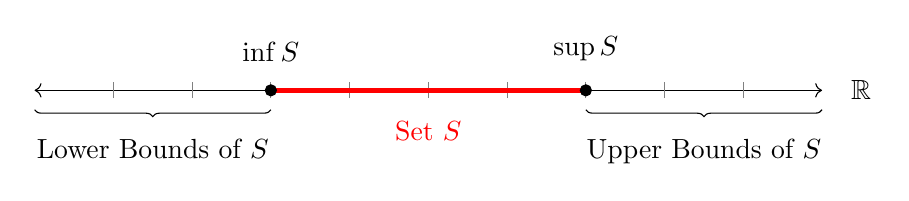
\begin{tikzpicture}
        \coordinate (setstart) at (-2, 0);
        \coordinate (setend) at (2, 0);
        \draw[<->] (-5, 0) -- (5, 0) node[right, xshift=7pt] {$ \mathbb{R} $};
        \draw[decoration={brace, mirror, raise=7pt}, decorate] (-5, 0) --
            (setstart) node[pos=0.5, anchor=north, yshift=-14pt]
            {Lower Bounds of $ S $};
        \draw[decoration={brace, mirror, raise=7pt}, decorate] (setend) --
            (5, 0) node[pos=0.5, anchor=north, yshift=-14pt]
            {Upper Bounds of $ S $};
        \foreach \i in {-4, ..., 4} \draw[gray] (\i, -.1) -- (\i, .1);
        \draw[ultra thick, red] (setstart) -- (setend) node[pos=0.5,
            anchor=north, yshift=-7pt]{Set $ S $};
        \filldraw (setstart) circle (2pt) node[above, yshift=7pt] {$ \inf S $};
        \filldraw (setend) circle (2pt) node[above, yshift=7pt] {$ \sup S $};
    \end{tikzpicture}
    \captionof{figure}{$ S \subset \mathbb{R} $  and its bounding points on the
        real line}
\end{definition}
\begin{definition}{Supremum and Infimum of  \texorpdfstring{$\emptyset$}{the Empty Set}}{sup-inf-empty}
Consider the empty set $\emptyset$.
\begin{equation}
    \sup(\emptyset)= -\infty \text{ and } \inf(\emptyset)=\infty
\end{equation}
This is the only set for which $\inf(S)>\sup(S)$
\end{definition}
\begin{definition}{The \texorpdfstring{$ \ell^\infty $}{Ell-Infinity}
        Set of Bounded Sequences}{ell-infinity}
    Consider $ \mathbb{R}^\mathbb{N} $: the set of all sequences of reals. We cannot work with this entire space, since many real sequences are unbounded,
    and the $ d_1 $ and $ d_2 $ canonical metrics give rise to non-finite sums.\\
    Therefore, we consider the set $ \ell^\infty $ as the \emph{set of
    all bounded real sequences}:
    \begin{equation}
        \vec{x} \in \ell^\infty \iff \exists M > 0 \text{ such that }
            \vert x_n \vert \leq M \text { for all } n \in \mathbb{N}.
    \end{equation}
    Then, the infinity metric is defined in terms of the supremum, since a
    sequence with infinite terms mightn't possess a maximum:
    \begin{equation}
        d_\infty(\vec{x}, \vec{y}) = \sup\left\{\vert x_i - y_i \vert \colon
            i \in \mathbb{N}\right\} \text { for } \vec{x}, \vec{y} \in \ell^\infty. 
    \end{equation}
\end{definition}
\begin{definition}{The Set of Bounded Functions}{bounded-functions-set}
    $ B([0,1]) $ is the \emph{set of all bounded functions} $ f $ such that
    $ f \colon [0, 1] \to \mathbb{R} $.
    
    A \emph{bounded function} $f(x)$ is such that $\exists M >0$ such that$\vert f(x) \vert \leq M $ for all $x \in$ the domain.
\end{definition}
\begin{definition}{The Set of Continuous Functions}{cts-functions-set}
    $ C([0,1]) $ is the \emph{set of all continuous functions} $ f $ such that
    $ f \colon [0, 1] \to \mathbb{R} $.
\end{definition}
\begin{theorem}{\texorpdfstring{$(B([0, 1]),d_\infty)$}{The set of bounded functions over 0 and 1 inclusive with the sup-metric} forms a metric space}{bounded-is-metric}
    Consider the $ d_\infty $ metric on $ B([0, 1]) $ defined in terms of the
    supremum, such that the upper bound needn't lie in the set:
    \begin{equation}
        d_\infty \colon B([0, 1]) \times B([0, 1]) \to [0, \infty)
            \text{ where } d_\infty(f, g) = \sup\left\{\vert f(t) - g(t) \vert
            \colon t \in [0, 1] \right\}.
    \end{equation}
    Then, $ \left(B([0, 1]),\, d_\infty\right) $ is a metric space.
    \begin{proof}
        We must verify that $ d_\infty : B([0, 1]) \times B([0, 1]) \to [0,
        \infty) $ satisfies the metric axioms described in
        \cref{definition:metric} for all $ f, g, h \in B([0, 1]) $.
        \begin{itemize}
            \item[(M1)] Since $ f, g $ are bounded functions with domain $[0,1]$ and co-domain $\mathbb{R}$, so $f-g$ is bounded. Thus,
                \begin{equation}
                    d_\infty(f,g)=\sup\{\vert f(t)-g(t)\vert\} \leq M
                \end{equation}
            but $\sup\{\vert f(t)-g(t)\vert\} \geq 0$, so $d_\infty(f,g)\geq 0$ for all $f,g$
               
            \item[(M2)] \iffforward If $ f = g $, then $ \vert f(t) - g(t) \vert = 0 $
                for all $ t \in [0, 1] $, so $ d_\infty(f, g) = \sup\{0, 0,
                \ldots\} = 0 $.

                \iffbackward Furthermore, if $ d_\infty(f, g) = 0 $, then we
                know that $ \sup\left\{ \vert f(t) - g(t) \vert \colon t \in [0,
                1] \right\} = 0 $. We know that $ \vert f(t) - g(t) \vert \geq 0
                $, so $ \vert f(t) - g(t) \vert = 0 $ follows immediately, from
                which we can conclude that $ f(t) = g(t) $ for all $ t \in [0,
                1] $, hence $ f = g $.

                Thus, $ d_\infty(f, g) = 0 \iff f = g $.
            \item[(M3)] By the symmetry of the standard metric on $ \mathbb{R} $, the
                symmetry of $ d_\infty $ on $ B([0, 1]) $ follows immediately:
                \begin{align}
                    d_\infty(f, g) &= \sup\left\{ \vert f(t) - g(t) \vert \colon
                        t \in [0, 1] \right\} \\
                    &= \sup\left\{ \vert g(t) - f(t) \vert \colon t \in [0, 1]
                        \right\} \\
                    &= d_\infty(g, f).
                \end{align}
            \item[(M4)] By the triangularity property of the standard metric on $
                    \mathbb{R} $,
                \begin{align}
                    d_\infty(f, g) &= \sup\left\{ \vert f(t) - g(t) \vert \colon
                        t \in [0, 1] \right\} \\
                    &= \sup\left\{ \vert f(t) - h(t) + h(t) - g(t) \vert \colon
                        t \in [0, 1] \right\} \\
                    &\leq \sup\left\{ \vert f(t) - h(t) \vert \colon t \in [0,
                        1] \right\} + \sup\left\{ \vert h(t) - g(t) \vert \colon
                        t \in [0, 1] \right\} \\
                    &= d_\infty(f, h) + d_\infty(h, g),
                \end{align}
                hence $ d_\infty $ possesses the property of triangularity on $
                B([0, 1]) $.
        \end{itemize}
        Thus, $ \left(B([0,1]), d_\infty\right) $ is a metric space.
    \end{proof}
\end{theorem}
\pagebreak


\lecture{Lecture III}{Viewer.aspx?id=afbe7e12-8494-4fe3-b73f-b08a009bdc46}{
    Lecture Three opens with a counterexample to challenge a common
    misconception. It continues to introduce the concept of \emph{norms} as
    generalisations of the absolute value function, \emph{metric subspaces}, and
    \emph{isometric maps}, complemented by a simple example.
}{\DTMdisplaydate{2023}{10}{03}{Tuesday}}

\begin{example}{Hemming Distance}{hemming-distance}
    Despite the examples seen thus far, metric spaces needn't support an
    associated arithmetic or algebraic structure.\\ For instance, let $ A =
    \{ 0, 1 \}^\mathbb{N} $ be the set of alphabet and $ A(N)$ be the set of all strings of length $N$. Then, we can define the Hemming distance $H : A(N) \rightarrow [0,\infty]$ to be the number of places where string $x$ differs from string $y$. For example,
    \begin{equation}
        H(010,110)=1
    \end{equation}
    Despite there being no inherent algebraic structure or ordering on $A(n)$,$H$ is a metric that provides a notion of \emph{distance}.
\end{example}
\begin{definition}{Vector Spaces and Norm}{norm}
    A \emph{vector space} $ V $ is a non-empty set which roughly satisfy 
    \begin{equation}
        \mu\vec{u} +\lambda\vec{v}\in V \text{ if } \vec{u},\vec{v} \in V \text{ and } \mu,\lambda\in \mathbb{R} \text{ or } \mathbb{C} 
    \end{equation}
    A \emph{norm} is an abstraction of the absolute value. Suppose that $ V $ is
    a normable vector space. Then $ \vert\vert\cdot\vert\vert \colon V \to
    \mathbb{R} $ is such that, for all $ \vec{x}, \vec{y} \in V $,
    \setaxiomprefix{N}
    \begin{axioms}
        \item $ \vert\vert \vec{x} \vert\vert \geq 0 $;
        \item $ \vert\vert \vec{x} \vert\vert = 0 \iff \vec{x} = \vec{0} $;
        \item $ \vert\vert \lambda \vec{x} \vert\vert = \vert \lambda \vert
            \vert\vert \vec{x} \vert\vert $ for all $ \lambda \in \mathbb{R} $;
        \item $ \vert\vert \vec{x} + \vec{y} \vert\vert \leq \vert\vert \vec{x}
            \vert\vert + \vert\vert \vec{y} \vert\vert $.
    \end{axioms}
    $ V $ equipped with $ \vert\vert \cdot \vert\vert $ is a \emph{normed
    space}. Note that any norm can give rise to a metric; such a metric is
    sometimes called the \emph{metric induced by the norm}.
\end{definition}
\begin{definition}{Metric Subspace}{metric-subspace}
    Let $(X,d)$ be a metric space.\\
    We can consider $A \subseteq X$ to be a \emph{metric subspace} by restricting $d$ to $A\times A$. That is
    \begin{equation}
        d\vert_A: A \times A \rightarrow [0,\infty)
    \end{equation}
\end{definition}
When is the metric space $(X,d)$ the ``same" as $(Y,\hat{d})$?\\
Perhaps, the most rigid ``same" is an isometry.
\begin{definition}{Isometric Map}{isometric-map}
    Suppose that $ (X, d) $ and $ (Y, \hat{e}) $ are metric spaces.\\
    We say that $X$ is \emph{isometric} to $Y$ if and only if $\exists$ $\phi
    \colon X \to Y $ which is surjective and 
    \begin{equation}
        \hat{d}(\phi(a), \phi(b)) = d(a, b) \text{ for all } a, b \in X
    \end{equation}
    The function $\phi$ is called an \emph{isometric mapping}.
\end{definition}
\begin{example}{\texorpdfstring{$\mathbb{R}^2$ is isometric to $\mathbb{C}$}{Complex Isometry}}{complex-isometry}
    There exists a surjective (bijective) function $\phi$, where
    \begin{align*}
        \phi : \mathbb{R}^2 \rightarrow \mathbb{C}\\
        \phi(x,y)= x+iy
    \end{align*}
    Also, 
    \begin{align*}
        d(\phi(x,y),\phi(x',y')) &= \vert (x+iy)-(x'-iy')\vert \\
        &= \vert (x+x')+(y-y')\vert\\
        &= \sqrt{(x+x')^2+(y-y')^2}\\
        &= \vert (x,y)-(x',y')\vert\\
        &= d((x,y),(x',y'))
    \end{align*}
    Hence, $\mathbb{R}^2$ qualifies as an isometry to $\mathbb{C}$.
\end{example}
\pagebreak

\lecture{Lecture IV}{Viewer.aspx?id=3a47174e-ed9d-413d-b309-b08c009bdb8e}{
    Lecture Four begins an investigation into the geometry of a metric space. In
    particular, we introduce \emph{open and closed balls}, \emph{interior
    points}, \emph{boundary points}, and \emph{exterior points}, and define
    \emph{open} and \emph{closed} sets in terms of these concepts. We take an
    example metric space and rigorously compute its interior, boundary, and
    exterior, and finally show (by example) that considering objects as either
    subsets or subspaces can vastly alter their topological properties.
}{\DTMdisplaydate{2023}{10}{05}{Thursday}}

\begin{definition}{Open and Closed Balls}{balls}
    Suppose that $ (X, d) $ is a metric space, and that $ x_0 \in X $. For every
    $ \epsilon > 0 $, we define the \emph{open ball centered at $ x_0 $ with
    radius $ \epsilon $} to be the set $ B(x_0, \epsilon) = \left\{ x \in X
    \colon d(x, x_0) < \epsilon \right\} $. Analogously, the \emph{closed ball
    centered at $ x_0 $ with radius $ \epsilon $} is defined to be the set
    $ \overline{B}(x_0, \epsilon) = \left\{ x \in X \colon d(x, x_0) \leq
    \epsilon \right\} $.

    \centering
    \begin{minipage}{.5\linewidth}
        \centering
        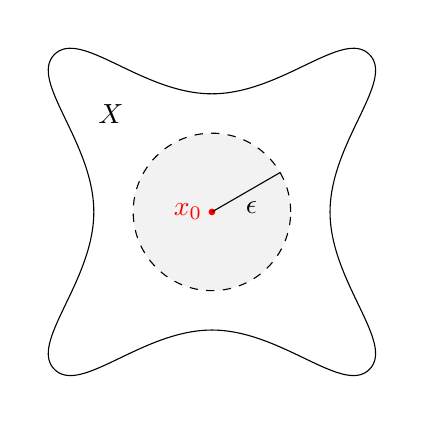
\begin{tikzpicture}
            \pic at (0, 0) {squarespace};
            \draw[fill=ballfill, dashed] (0, 0) circle[radius=1] node[above
                left=1cm]{$ X $};
            \filldraw[red] (0, 0) circle (1pt) node[left] {$ x_0 $};
            \draw (0, 0) -- ++(30:1cm) node[anchor=north, pos=0.5, xshift=2pt]
                {$ \epsilon $};
        \end{tikzpicture}
        \captionof{figure}{The open ball $ B(x_0, \epsilon) \subset X $}
    \end{minipage}\hfill
    \begin{minipage}{.5\linewidth}
        \centering
        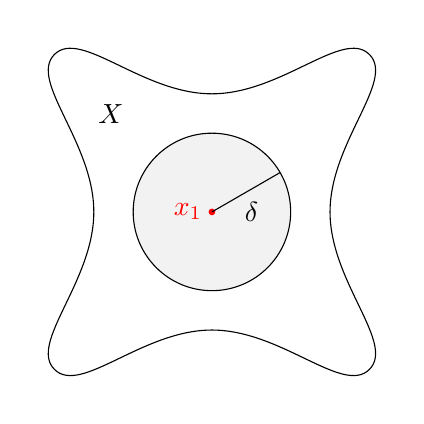
\begin{tikzpicture}
            \pic at (0, 0) {squarespace};
            \draw[fill=ballfill] (0, 0) circle[radius=1] node[above left=1cm]
                {$ X $};
            \filldraw[red] (0, 0) circle (1pt) node[left] {$ x_1 $};
            \draw (0, 0) -- ++(30:1cm) node[anchor=north, pos=0.5, xshift=2pt]
                {$ \delta $};
        \end{tikzpicture}
        \captionof{figure}{The closed ball $ \overline{B}(x_1, \delta)
            \subset X $}
    \end{minipage}
\end{definition}
\begin{definition}{Interior Points}{interior-points}
    Let $ A \subset X $. An \emph{interior point} $ y \in X $ of $ A $ is an
    element for which $ B(y, \epsilon) \subset A $ for some $ \epsilon > 0 $.
    That is, there is an open ball centred at $ y $ with radius $ \epsilon $
    that is completely contained within $ A $. The set of all such points is
    denoted as $ A^o $, and is called \emph{the interior of $ A $}.
\end{definition}
\begin{definition}{Boundary Points}{boundary-points}
    The element $ y \in X $ is a \emph{boundary point} of $ A $ if and only if
    for any $ \epsilon > 0 $, $ B(y, \epsilon) \cap A \neq \emptyset $ and
    $ B(y, \epsilon) \cap A^c \neq \emptyset $. That is, any open ball centred
    at $ y $ always intersects with $ A $ and its complement $ A^c $. The set of
    all such points is denoted as $ \partial A $, and is called \emph{the
    boundary of $ A $}.
\end{definition}
\begin{definition}{Exterior Points}{exterior-points}
    The element $ y \in X $ is an \emph{exterior point} of A if and only if for
    some $ \epsilon > 0 $, $ B(y, \epsilon) \subset A^c $. That is, there exists
    an open ball centred at $ y $ which intersects only with the complement of
    $ A $; this can also be interpreted as an interior point of the complement.
    The set of all such points is denoted as $ A^e $, and is called \emph{the
    exterior of A}.
\end{definition}
\begin{example}{Illustration of Interior, Boundary, and Exterior Points}
        {int-bound-ext-graphic}
    Consider an ambient space $ X $, and the shaded subset $ A \subseteq X $.
    We can illustrate examples of points from the interior, boundary, and
    exterior of $ A $.

    \begin{minipage}{.3\linewidth}
        \centering
        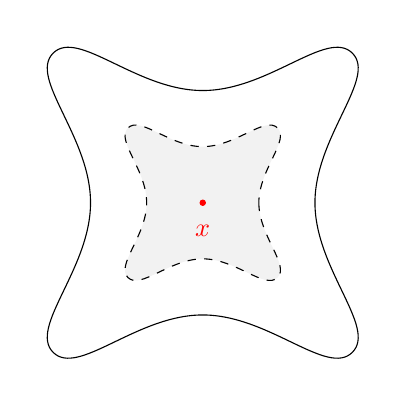
\begin{tikzpicture}[scale=0.95]
            \pic at (0, 0) {squarespace};
            \pic[scale=0.5, every path/.style={fill=ballfill, dashed}] at (0, 0)
                {squarespace};
            \filldraw[red] (0, 0) circle (1pt) node[below, yshift=-5pt] {$ x $};
        \end{tikzpicture}
        \captionof{figure}{An interior point $ x \in A^o $}
    \end{minipage}\hfill
    \begin{minipage}{.3\linewidth}
        \centering
        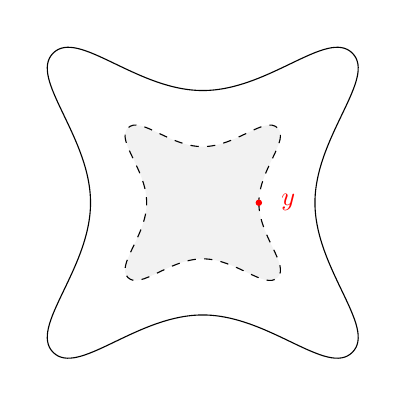
\begin{tikzpicture}[scale=0.95]
            \pic at (0, 0) {squarespace};
            \pic[scale=0.5, every path/.style={fill=ballfill, dashed}] at (0, 0)
                {squarespace};
            \filldraw[red] (.75, 0) circle (1pt) node[right, xshift=5pt]
                {$ y $};
        \end{tikzpicture}
        \captionof{figure}{A boundary point $ y \in \partial A $}
    \end{minipage}\hfill
    \begin{minipage}{.3\linewidth}
        \centering
        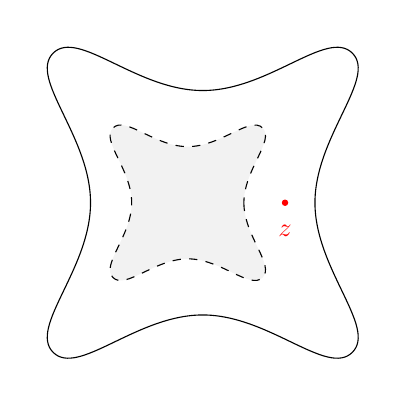
\begin{tikzpicture}[scale=0.95]
            \pic at (.2, 0) {squarespace};
            \pic[scale=0.5, every path/.style={fill=ballfill, dashed}] at (0, 0)
                {squarespace};
            \filldraw[red] (1.3, 0) circle (1pt) node[below, yshift=-5pt]
                {$ z $};
        \end{tikzpicture}
        \captionof{figure}{An exterior point $ z \in A^e $}
    \end{minipage}

    Note that the interior, boundary, and exterior are mutually disjoint and can
    be placed under the disjoint union operation to form the entire ambient
    space. This fact is henceforth denoted by ``$ A^o \coprod \partial A \coprod
    A^e = X $'' for $ A \subseteq X $.
\end{example}
\begin{example}{Finding the interior, boundary, and exterior of a set}{int-bound-ext}
    Consider $ (\mathbb{R}, d) $ with $ A = (0, 1] \subset \mathbb{R} $.
    Intuitively, we can conjecture that $ A^o = (0, 1) $, $ \partial A = \{0,
    1\} $, and $ A^e = \mathbb{R} \setminus (0, 1) = (-\infty, 0) \cup (1,
    \infty) $, however these claims must be proven rigorously by (a) showing
    that the conjectured points do belong to the relevant set, and (b) showing
    that the conjectured points are the only elements to belong to the relevant
    set.
    \begin{itemize}
        \item First consider the interior. Take $ x \in (0, 1) $. By
            \cref{definition:interior-points}, we want to show that there is an
            $ \epsilon > 0 $ such that $ B(x, \epsilon) \subset (0, 1] = A $.
            Set $ \epsilon_1 \coloneq x $, and $ \epsilon_2 \coloneq 1-x $.
            Given that $ 0 < x < 1 $, we can take an $ \epsilon \coloneq
            \min\{ \epsilon_1, \epsilon_2 \} $. Then, since $ \epsilon/2 <
            \epsilon_1, \epsilon_2 $,
            \begin{equation}
                B(x, \epsilon/2) = \left\{ y \in \mathbb{R} \colon d(x, y) <
                    \epsilon/2 \right\} \subset A.
            \end{equation}
            This proves that $ (0, 1) \subseteq A^o $.

            We now need to eliminate the remaining candidates in $ \mathbb{R}
            \setminus (0, 1) $ from having possible membership in $ A^o $. The
            points $ x < 0 $ and $ x > 1 $ can be discarded immediately, since
            any open ball centred at these points could never lie totally within
            $ A $, due to their positive radii $ \epsilon $. Finally, we need to
            show that $ \{0,1\} \not\subset A^o $. Without loss of generality,
            pick $ x = 1 $, and take an $ \epsilon > 0 $ to consider the open
            ball $ B(x, \epsilon) $. Any such ball would contain a point that is
            strictly greater than 1, and hence would contain points outside of $
            A $. Thus, $ x \not\in A^o $, and $ A^o = (0, 1) $ as claimed.
        \item Now consider the boundary, as described in
            \cref{definition:boundary-points}. We claim that $ \{0, 1\} =
            \partial A $, and first demonstrate that $ \{0, 1\} \subseteq
            \partial A $.  Without loss of generality, we show that $ 0 \in
            \partial A $. Let $ \epsilon > 0 $, and consider $ B(0, \epsilon) =
            (-\epsilon, \epsilon) $. Clearly, since $ \epsilon > 0 $, $
            (-\epsilon, \epsilon) \cap A \neq \emptyset $ and $ (-\epsilon,
            \epsilon) \cap A^c \neq \emptyset $; thus, $ 0 $ is a boundary
            point.

            Now, we show that there are no other boundary points of $ A $ in $
            \mathbb{R} $. We know that $ \mathbb{R} = A^o \coprod \partial A
            \coprod A^e $, hence $ A^o \cap \partial A = \emptyset $, thus $ (0,
            1) \not\subset \partial A $. Without loss of generality for $ x < 0
            $, consider points $ x > 1 $. Therefore, there exists an $ \epsilon
            > 0 $ such that $ x = 1 + \epsilon $. Considering $ B(x, \epsilon/2)
            $, we can see that $ B(x, \epsilon/2) \subset A^c $, which implies
            that $ B(x, \epsilon/2) \cap A = \emptyset $. Thus, $ \{ 0, 1 \} =
            \partial A $.
        \item Finally, consider the exterior, as described in
            \cref{definition:exterior-points}. Recall that the entire space can
            be expressed as a disjoint union, e.g. $ \mathbb{R} = A^o \coprod
            A^e \coprod \partial A $. Hence,
            \begin{align}
                A^e &= \mathbb{R} \setminus \left( A^o \cup \partial A
                    \right) \\
                &= \mathbb{R} \setminus [0, 1] \\
                &= (-\infty, 0) \cup (1, \infty),
            \end{align}
            as conjectured.
    \end{itemize}
\end{example}
\begin{theorem}{Boundaries of the empty set and entire metric space}{bound-empty-metric}
For an empty set $\emptyset$, its set of boundary points $\partial \emptyset = \emptyset$. \\
For a metric space $(X,d)$, its set of boundary points $\partial X = \emptyset$.
\end{theorem}
\begin{definition}{Open, Closed, and Clopen Sets}{open-closed-clopen-sets}
    Let $ (X, d) $ be a metric space. A subset $ A $ of $ X $ is \emph{open} if
    and only if $ A \cap \partial A = \emptyset $.\\ 
    A subset $ F $ of $ X $ is
    \emph{closed} if and only if $ \partial F \subseteq F $.\\
    Note that a set can
    be both open and closed: typical examples are the empty set and the entire
    space; these sets are called \emph{clopen}.

    \centering
    \begin{minipage}{.5\linewidth}
        \centering
        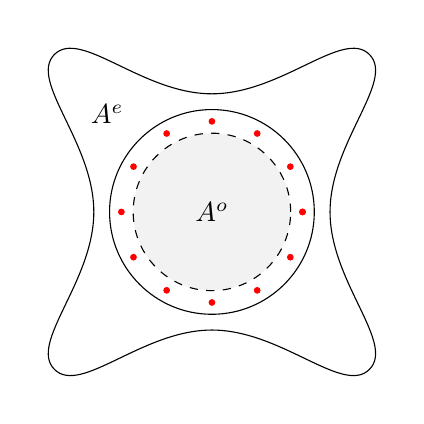
\begin{tikzpicture}
            \pic at (0, 0) {squarespace};
            \draw[fill=ballfill, dashed] (0, 0) circle[radius=1];
            \draw (0, 0) circle[radius=1.3] node {$ A^o $} node[above left=1cm]
                {$ A^e $};
            \foreach \angle in {0, 30, ..., 360}
                \filldraw[red] (\angle:1.15cm) circle (1pt);
        \end{tikzpicture}
        \captionof{figure}{An open set $ A $ does not contain its boundary
            points.}
    \end{minipage}\hfill
    \begin{minipage}{.5\linewidth}
        \centering
        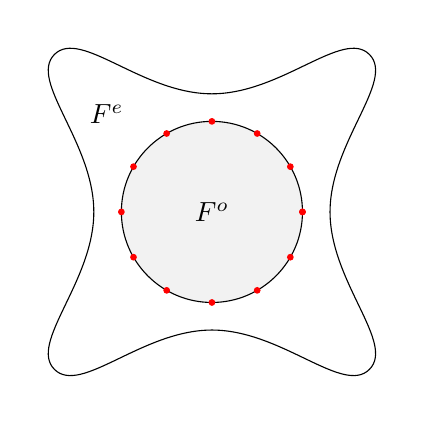
\begin{tikzpicture}
            \pic at (0, 0) {squarespace};
            \draw[fill=ballfill] (0, 0) circle[radius=1.15] node {$ F^o $}
                node[above left=1cm] {$ F^e $};
            \foreach \angle in {0, 30, ..., 360}
                \filldraw[red] (\angle:1.15cm) circle (1pt);
        \end{tikzpicture}
        \captionof{figure}{A closed set $ F $ contains its boundary points.}
    \end{minipage}
\end{definition}
\begin{theorem}{Interior, Boundary and Exterior of a subspace}{subset-subspace}
    For any sub-space $A$ of $X$, its interior $A^o = A$  and its boundary $\partial A =$ its exterior $A^e=\emptyset$. 
    \begin{proof}
        For any sub-space, its ``view" is restricted to $A$. Therefore its complement $A^c = \emptyset$.\\
        This means that no boundary point $\partial A$ can exist, since the intersection of the ball $B(x, \epsilon)$, where $x \in \partial A$, with $A^c$ will always be empty.\\
        It also follows that $A^e$ is empty and so $A^o = A$.
    \end{proof}
\end{theorem}
\pagebreak

\lecture{Lecture V}{Viewer.aspx?id=dbcb156d-d828-454f-929d-b091009bf65b}{
    Lecture Five proves multiple important theorems: a set is open if and only
    if its complement is closed; a set is open if and only if we can place an
    open ball around every point and stay inside of the set; and an open set can
    be expressed as a union of open balls. We also introduce the notion of
    \emph{a topology} $ T_d $ as the collection of all open subsets, and prove
    theorems related to closure under the familiar union and intersection set
    operations.
}{\DTMdisplaydate{2023}{10}{10}{Tuesday}}

\begin{theorem}{A subset is open if and only if its complement is closed}{open-subset-closed-complement}
    Consider a set $ A \subseteq X $. Then, $ A $ is open if and only if $ A^c $
    is closed.
    \begin{proof}
        This can be proven by unravelling the definitions of open and closed
        sets (\cref{definition:open-closed-clopen-sets}) and boundary points
        (\cref{definition:boundary-points}).

        \iffforward First, suppose that $ A $ is open.  If $ A = \emptyset $,
        then $ A^c = X $. The entire space is known to be clopen, and thus
        closed.\\
        If $ A \neq \emptyset $, then $ A \cap \partial A = \emptyset $,
        and $ \partial A \subseteq A^c $.  We can now see a useful equality by
        using the fact that $ \left(A^c\right)^c = A $:
        \begin{align}
            \partial \left(A^c\right) &= \left\{ y \in X \colon \forall \epsilon
                > 0 \, B(y, \epsilon) \cap A^c \neq \emptyset \land B(x,
                \epsilon) \cap \left(A^c\right)^c \neq \emptyset \right\}%
                \label{eqn:boundary-complement-boundary-first}\\
            &= \left\{ y \in X \colon \forall \epsilon > 0 \, B(y, \epsilon)
                \cap A^c \neq \emptyset \land B(x, \epsilon) \cap A \neq
                \emptyset \right\} \\
            &= \partial A.\label{eqn:boundary-complement-boundary-last}
        \end{align}
        Since $ \partial A \subseteq A^c $, and $ \partial A = \partial
        \left(A^c\right) $, we know that $ \partial \left(A^c\right) \subseteq
        A^c $. Hence, $ A^c $ is closed.

        \iffbackward Next, assume that $ A^c $ is closed, hence $ \partial
        \left(A^c\right) \subseteq A^c $. Given that $ \partial A = \partial
        \left(A^c\right) $, $ \partial A \subseteq A^c $. Since $ A^c \cap A =
        \emptyset $, we know that $ \partial A \cap A = \emptyset $, and thus $
        A $ is open.
    \end{proof}
\end{theorem}
\begin{definition}{The topology of a metric space}{topology}
    The \emph{topology} of a metric space $ (X, d) $, denoted as $ T_d $,
    is defined to be \emph{the collection of all open subsets of $ X $}. Note
    that since $ T_d \subseteq \mathcal{P}(X) $ for any set $ X $, so $ T_d \neq \emptyset $ as $ \emptyset,
    X \in T_d $, .
\end{definition}
\begin{theorem}{Equivalence between openness and the existence of open balls}
        {openness-open-balls}
    Let $ A \subseteq X $ be open. Then, every point of $ A $ is an interior
    point of A. Equivalently, $ A $ is open if and only if there is an open ball
    around every point in $ A $ that resides within $ A $:
    \begin{equation}
        \forall x \in A\, \exists \epsilon > 0 \text{ such that } B (x,
        \epsilon) \subseteq A.
    \end{equation}

    \begin{minipage}{\dimexpr.6\linewidth-2em}
        \begin{proof}
            \iffforward First assume that $ A $ is open. By definition, $ A \cap
            \partial A = \emptyset $.\\
            If $ A = \emptyset $, then there exists no
            points to select, and the universal quantifier cannot select any
            points for $ x $. \\
            If $ A \neq \emptyset $, then there must be at
            least one $ \epsilon > 0 $ such that $ B(x, \epsilon) \subseteq A $
            or $ B(x, \epsilon) \subseteq A^c $ for any $ x \in A $. But, since
            $ x \in A $, it is not possible that $ B(x, \epsilon) $ is entirely
            contained within $ A^c $, since $ x \in B(x, \epsilon) $. Hence, $
            B(x, \epsilon) \subseteq A$, as required.

            \iffbackward Next, suppose that $ \forall x \in A\, \exists \epsilon
            > 0 $ such that $ B (x, \epsilon) \subseteq A $. Take any $ x \in A
            $.  Immediately, we can see that $ x \not\in \partial A $, since $
            B(x, \epsilon) \cap A^c = \emptyset $, because $ B(x, \epsilon)
            \subseteq A $. Hence, $ A $ is open.
        \end{proof}
    \end{minipage}\hfill
    \begin{minipage}{.4\linewidth}
        \centering
        \begin{tikzpicture}
            \coordinate (x1point) at (1, 1);
            \coordinate (x2point) at (-1, 1);
            \coordinate (x3point) at (0, -1);
            \draw[dashed] (0, 0) circle (2.7cm);
            \foreach \pt in {1, 2, 3}{
                \filldraw[red] (x\pt point) circle (1pt);
                \draw[dashed, red] (x\pt point) circle (.4cm*\pt+.05cm)
                    node[below] {$ x_\pt $};
                \draw[red] (x\pt point) -- ++(45*\pt:.4cm*\pt+.05cm);
            }
        \end{tikzpicture}
        \captionof{figure}{Every point supports an open ball}
    \end{minipage}
\end{theorem}
\begin{definition}{Definitions of open}{open-def}
    For any set $A\subseteq X$, its openness can be defined in multiple ways:
    \begin{equation}
        \begin{split}
        A \text{ is open} &\iff A^c \text{ is closed}\\
        &\iff \partial A\cap A = \emptyset\\
        &\iff \text{For any }x\in A, \exists \epsilon > 0, \text{ such that } B(x, \epsilon) \subseteq A
    \end{split}
    \end{equation}
\end{definition}
\begin{theorem}{The open ball is open}{open-ball-open}
    For any $ x \in X $ and any $ \epsilon > 0 $, $ B(x, \epsilon) \in T_d $.
    Since $ T_d $ is defined to be a collection of open sets, this statement is
    equivalent to the claim that ``\emph{the open ball is open}''.
    \begin{proof}
        Take an $ x \in X $ and construct the open ball $ B(x, \epsilon) $, for
        a fixed $ \epsilon > 0 $. Take $ y \in B(x, \epsilon) $ and let $ \Delta
        \coloneq d(x, y) $.\\
        If $ x=y $, then $ B(x, \epsilon) = B(y, \epsilon)
        \subseteq B(x, \epsilon) $, there is nothing to do.\\ Therefore, we assume
        that $ x \neq y $, thus $ \Delta > 0 $ and $ 0 < \Delta < \epsilon $.
        Let $ \epsilon^\prime \coloneq \min\left\{ \Delta, \epsilon-\Delta
        \right\} $ and consider $ B(y, \epsilon^\prime/2) $.

        \begin{minipage}{.45\linewidth}
            To show the openness of the open ball, it is sufficient to show that
            $ B(y, \epsilon^\prime/2) \subseteq B(x, \epsilon) $, as it would satisfy \cref{theorem:openness-open-balls}.\\
            By the
            triangle inequality on $ d $, for any $ z \in B(y,
            \epsilon^\prime/2) $,
            \begin{align}
                d(x, z) &\leq d(x, y) + d(y, z) \\
                &\leq \Delta + \epsilon^\prime/2 \\
                &= \Delta + \min\left\{\Delta, \epsilon-\Delta\right\}/2 \\
                &\leq \Delta + (\epsilon-\Delta)/2 \\
                &< \Delta + \epsilon - \Delta \\
                &= \epsilon
            \end{align}
        \end{minipage}\hfill
        \begin{minipage}{.5\linewidth}
            \centering
            \begin{tikzpicture}
                \coordinate (xpoint) at (0, 0);
                \coordinate (ypoint) at (0, 1.5);
                \draw[dashed] (xpoint) circle (2.7cm);
                \draw (xpoint) -- ++(-30:2.7cm) node[anchor=south, pos=0.5,
                    xshift=3pt, yshift=3pt] {$ \epsilon $};
                \filldraw[blue] (xpoint) circle (1pt) node[left, xshift=-3pt]
                    {$ x $};
                \filldraw[red] (ypoint) circle (1pt) node[right, xshift=3pt]
                    {$ y $};
                \draw[blue, dotted] (xpoint) -- (ypoint);
                \draw[dashed, red] (ypoint) circle (1cm);
                \draw[red] (ypoint) -- ++(120:1cm) node[left, pos=.5,
                    yshift=-3pt] {$ \frac{\epsilon^\prime}{2} $};
                \node[blue] at (-.75, -1.3)
                    {$ \left[\,\Delta = d(x, y)\,\right] $};
            \end{tikzpicture}
            \captionof{figure}{Careful construction of
                $ B(y, \epsilon^\prime/2) $}
        \end{minipage}

        Thus, $ z \in B(x, \epsilon) $ for all $ z \in B(y, \epsilon^\prime/2)
        $. Therefore, $ B(y, \epsilon^\prime/2) \subseteq B(x, \epsilon) $, and
        open balls are indeed open.
    \end{proof}
\end{theorem}
\begin{theorem}{Elements of the topology are unions of open balls}
        {topology-open-balls}
    If $ A \in T_d $ and $ A \neq \emptyset $, then $ A $ is a union of open
    balls.
    \begin{proof}
        Suppose that $ A \neq \emptyset $ and is open. Take any $ x \in A $, and
        we know by \cref{theorem:openness-open-balls} that there exists an $
        \epsilon > 0 $ such that $ B(x, \epsilon) \subseteq A $. \\
        Then, we claim
        that
        \begin{equation}
            A = \bigcup_{x \in A} B\left(x, \epsilon(x)\right)
            \underbrace{\iff \left[
                A \subseteq \bigcup_{x \in A} B\left(x, \epsilon(x)\right)
                    \,\land\, A \supseteq \bigcup_{x \in A} B\left(x,
                    \epsilon(x)\right)
                \right]}_{\text{true by the principle of double-inclusion}}.
        \end{equation}
        The leftmost conjunctive on the right-hand-side is clearly true: by
        placing an open ball of strictly positive radius around every point in $
        A $, the entire set will be covered, since $ x \in B(x, \epsilon) $ for
        any $ x $ and $ \epsilon > 0 $.\\
        The rightmost conjunctive is also true,
        since each individual ball is wholly contained within $ A $, and taking
        the union of all such interior balls cause any elements to ``escape''
        the set in which they reside. Hence, $ A $ is the union of the open
        balls centered about every point in $ A $.
    \end{proof}
\end{theorem}
\begin{theorem}{Any union of open sets is open}{open-union-open}
    Take \emph{any} (finite, countably infinite, or uncountable) collection of
    open sets $ \Lambda \subseteq T_d $. Then, for any $ \Lambda $,
    \begin{equation}
        \bigcup_{\Omega \in \Lambda} \Omega \in T_d \text { is open.}
    \end{equation}
    \begin{proof}
        Take a point $ x \in \bigcup_{\Omega \in \Lambda} \Omega $. Thus, there exists
        an open $ \Omega(x) $ such that $ x \in \Omega(x) $. By
        \cref{definition:open-closed-clopen-sets}, there exists an $ \epsilon >
        0 $ such that $ B(x, \epsilon) \subseteq \Omega(x) $. By transitivity,
        $ B(x, \epsilon) \subseteq \bigcup_{\Omega \in \Lambda} \Omega $, and
        every union of open sets is open by \cref{theorem:topology-open-balls}.
    \end{proof}
\end{theorem}
\begin{example}{Non-finite open sets are not closed under intersection}
        {non-finite-intersection-counterexample}
    Take $ (\mathbb{R}, d) $ and consider $ I_n \coloneq \left(-1/n, 1/n\right)
    $. Under infinite intersection, we calculate the singleton:
    \begin{equation}
        \bigcap_{n=1}^\infty I_n = \{0\}.
    \end{equation}
    It is known that all singletons are not open---since any $ B(x, \epsilon) $
    with $ \epsilon > 0 $ would exceed the bounds of $ \{x\} $---despite each
    individual $ I_n $ being open. Thus, the union property shown in
    \cref{theorem:open-union-open} does not apply with such generality to
    intersections.

    \centering
    \begin{tikzpicture}
        \coordinate (linestart) at (-5, 0);
        \coordinate (lineend) at (5, 0);
        \draw[<->] (linestart) -- (lineend) node[right, xshift=7pt]
            {$ \mathbb{R} $}; % Number line
        \foreach \i in {1, ..., 5}{
            \draw (-4/\i, .2) arc[start angle=90, end angle=270, radius=.2];
                % Left arc
            \draw (4/\i, .2) arc[start angle=90, end angle=-90, radius=.2];
                % Right arc
            \draw[<->] (-4/\i, -\i*.5-.5) -- (4/\i, -\i*.5-.5); % Interval
            \node at (5, -\i*.5-.5) {$ I_{\i} $}; % Interval marker
            \draw[dotted] (-4/\i, -\i*.5-.5) -- (-4/\i, .2); % Left dotted line
            \draw[dotted] (4/\i, -\i*.5-.5) -- (4/\i, .2); % Right dotted line
        }
        \draw (0, .2) -- (0, -.2); % Zero marker
        \node at (0, .6) {$ 0 $}; % Zero label
        \node at (-4, .6) {$ -1 $}; % Negative-one marker
        \node at (4, .6) {$ 1 $}; % Positive-one marker
        \node[xshift=-5pt] at (-2, .6) {$ -1/2 $}; % Negative-one-half marker
        \node at (2, .6) {$ 1/2 $}; % Positive-one-half marker
    \end{tikzpicture}
    \captionof{figure}{Nested intersections $ I_1 $ through $ I_5 $}
\end{example}
\begin{theorem}{Any finite intersection of open sets is open}
        {open-intersection-open}
    Take \emph{any finite} collection of open sets $ \Omega_1, \ldots, \Omega_N
    \in T_d $. Then,
    \begin{equation}
        \bigcap_{i=1}^N \Omega_i \in T_d \text{ is open.}
    \end{equation}
    \begin{proof}
        If $ \bigcap_{i=1}^N \Omega_i = \emptyset $, then there is nothing
        further to show, since $ \emptyset $ is known to be open and thus a
        member of all topologies $ T_d $.\\
        We now assume that the intersection is
        non-empty, from which we take an element $ x $. Thus, there exists an $
        \epsilon_i > 0 $ for each $\Omega_i$ for which $ B(x, \epsilon_i) \subseteq \Omega_i $. Let
        $ \epsilon \coloneq \min\left\{ \epsilon_1, \ldots, \epsilon_N \right\}
        $; then, $ B(x, \epsilon) \subseteq B(x, \epsilon_i) \subseteq \Omega_i
        $ for any choice of $ i = 1, \ldots, N $. Therefore,
        \begin{equation}
            B(x, \epsilon) \subseteq \bigcap_{i=1}^N \Omega_i,
        \end{equation}
        since $ B(x, \epsilon) $ is a member of \emph{every} $ \Omega_i $. Hence
        we can place an open ball with positive radius around any point and stay
        within the intersection; it is therefore open.
    \end{proof}
    \centering
    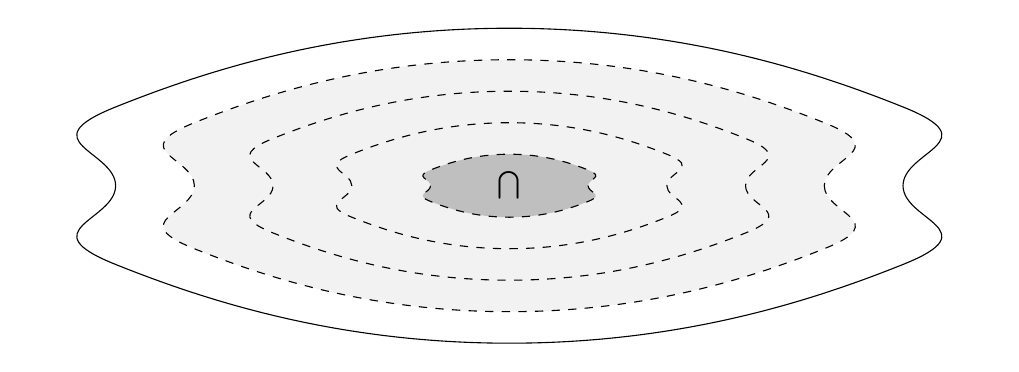
\begin{tikzpicture}
        \pic at (0, 0) {longspace};
        \foreach \i in {.8, .6, .4}{
            \pic[scale=\i, every path/.style={fill=ballfill, dashed}] at (0, 0)
                {longspace};
        }
        \pic[scale=.2, every path/.style={fill=lightgray, dashed}] at (0, 0)
            {longspace} node {$ \bigcap $};
    \end{tikzpicture}
    \captionof{figure}{We consider the intersection of open sets using the
        smallest open ball $ B(x, \epsilon) $.}
\end{theorem}
\begin{theorem}{Summary of \texorpdfstring{$ T_d $}{Open Set} Properties}
        {summary-open-set}
    Let $ (X, d) $ be a metric space, and let $ T_d $ be the topology induced by
    $ d $. Then,
    \setaxiomprefix{T}
    \begin{axioms}
        \item $ \emptyset, X \in T_d $;
        \item For any collection of open sets $ \Lambda \subseteq T_d $,
            $ \bigcup_{\Omega \in \Lambda} \Omega \in T_d $ is open
            (\cref{theorem:open-union-open});\label{axiom:open-union-open}
        \item For any finite collection of open sets $ \Omega_1, \ldots,
            \Omega_N \in T_d $, $ \bigcap_{i=1}^N \Omega_i \in T_d $ is open
            (\cref{theorem:open-intersection-open}).
    \end{axioms}
\end{theorem}
\pagebreak

\lecture{Lecture VI}{Viewer.aspx?id=ed63db50-27cd-4d84-8e60-b093009be8af}{
    Lecture Six continues to cover the topology induced by a metric by deriving
    the corresponding properties of closed sets. We introduce the concept of
    \emph{topological equivalence} as weaker method of determining ``sameness''
    between metric spaces. We finally define the \emph{closure} of a set, and
    prove that the closure is closed.
}{\DTMdisplaydate{2023}{10}{12}{Tuesday}}

\begin{theorem}{Summary of Closed Set Properties}{summary-closed-set}
    We can easily derive a dual of \cref{theorem:summary-open-set} for arbitrary
    and finite collections of \emph{closed} sets.
    \setaxiomprefix{F}
    \begin{axioms}
        \item For any collection of closed sets $ \mathcal{F} $,
            \begin{equation}
                \text{For all } F \in \mathcal{F} \text{, } \underbrace{F^c \in
                T_d}_\mathrm{\Cref{theorem:open-subset-closed-complement}}
                \implies\underbrace{\bigcup_{F \in \mathcal{F}} \left( F^c
                \right) \in T_d}_\mathrm{\Cref{axiom:open-union-open}} \implies
                \bigcap_{F \in \mathcal{F}} F \text { is closed,}
            \end{equation}
            since $ \left(\bigcap_{F \in \mathcal{F}}\right)^c =
            \bigcup_{F \in \mathcal{F}} \left( F^c \right) \in T_d $ by De
            Morgan's laws.
        \item Similarly, for any finite collection of closed sets $ F_1, \ldots,
            F_N $,
            \begin{equation}
                \left( \bigcup_{i=1}^N F_i \right)^c = \bigcap_{i=1}^N F_i^c \in
                T_d \implies \bigcup_{i=1}^N F_i \text{ is closed.}
            \end{equation}
    \end{axioms}
\end{theorem}
\begin{definition}{Topological Equivalence}{topological-equivalence}
    Let $ d $ and $ d^* $ be metrics on a set $ X $. Then, $ (X, d) $ and $ (X,
    d^*) $ are \emph{(topologically) equivalent} if and only if $ T_d = T_{d^*}
    $; that is, $ d $ and $ d^* $ induce the same topologies.
\end{definition}
\begin{theorem}{Determining Topological Equivalence}{determining-top-eq}
    Let $ X $ be a set and let $ d $ and $ d^* $ be metrics on $ X $. Then, $
    T_d = T_{d^*} $ if and only if there exists a scalar $ \lambda > 0 $ for
    which
    \begin{equation}
        \frac{1}{\lambda} d(x, y) \leq d^*(x, y) \leq \lambda d(x, y)
    \end{equation}
    for all $ x, y \in X $.
\end{theorem}
\begin{example}{\texorpdfstring{$ \mathbb{R}^2 $}{The plane} is topologically equivalent under the \texorpdfstring{$ d_1 $, $ d_2 $, and $ d_\infty $}{standard} metrics}{plane-top-eq}
    Recall the unit circles $ S^1_1 $ (\cref{fig:d1-unit-circle}), $ S_2^1 $
    (\cref{fig:d2-unit-circle}), and $ S_\infty^1 $
    (\cref{fig:dinf-unit-circle}) from \cref{example:unit-circles}. We claim
    (and give an information demonstration to show) that $ T_{d_1} = T_{d_2} =
    T_{d_\infty} $; that is, $ d_1 $, $ d_2 $, and $ d_\infty $ are
    topologically equivalent by \cref{definition:topological-equivalence}.

    We first consider the set $ S_1^1 \eqcolon \Omega $ in the space $
    \left(\mathbb{R}^2, d_2\right) $. Take a point $ x_0 \in \Omega $ and
    construct the open ball $ B(x_0, \epsilon/2) \subseteq S_1^1 $; such a ball
    can be created by considering an $ \epsilon \coloneq \min\left\{ \epsilon_1,
    \epsilon_2, \epsilon_3, \epsilon_4 \right\} $, where $ \epsilon_i $ for $ i
    = 1, 2, 3, 4 $ are the perpendicular distances from $ x_0 $ to the boundary
    of $ \Omega $ by the $ d_2 $ metric. Then, $ \Omega \in T_{d_2} $.

    Next, consider $ S_2^1 \eqcolon \Lambda $ in the space $ \left(\mathbb{R}^2,
    d_1\right) $. Constructing open balls in $ d_1 $ around the points in $
    \Lambda $ is easier still, since we only need to consider `diamonds' which
    lie entirely within the Euclidean $ d_2 $ unit circle. By covering the
    entire set, we can conclude that $ \Lambda \in T_{d_1} $.

    Intuitively, we can see that the metrics $ d_1 $ and $ d_2 $ induce the same
    topologies; an analogous argument applies for establishing the equivalences
    to $ d_\infty $.

    \centering
    \begin{minipage}{.45\linewidth}
        \centering
        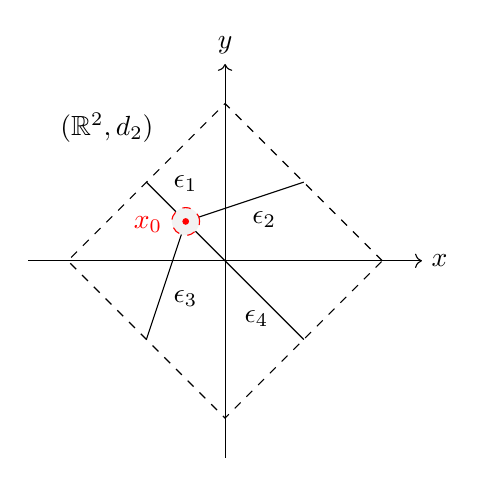
\begin{tikzpicture}
            \coordinate (x0point) at (-.5, .5);
            \draw[->] (-2.5, 0) -- (2.5, 0) node[right] {$x$};
            \draw[->] (0, -2.5) -- (0, 2.5) node[above] {$y$} node[left=1.5cm,
                below=.5cm] {$ (\mathbb{R}^2, d_2) $};
            \node[diamond, dashed, draw, minimum width=4cm, minimum height=4cm]
                {};
            \draw (x0point) -- (-1, 1) node[above, pos=.5, xshift=7pt]
                {$ \epsilon_1 $};
            \draw (x0point) -- (1, 1) node[below, pos=.5, xshift=7pt]
                {$ \epsilon_2 $};
            \draw (x0point) -- (-1, -1) node[below, pos=.5, xshift=7pt]
                {$ \epsilon_3 $};
            \draw (x0point) -- (1, -1) node[below, pos=.6, yshift=-3pt]
                {$ \epsilon_4 $};
            \draw[red, dashed, fill=ballfill] (x0point) circle (5pt);
            \filldraw[red] (x0point) circle (1pt) node[left, red, xshift=-5pt,
                yshift=-1pt] {$ x_0 $};
        \end{tikzpicture}
        \captionof{figure}{Considering the $ d_1 $-defined unit circle $ \Omega
            $ as an open set in the $ \left(\mathbb{R}^2, d_2\right) $ space.}
    \end{minipage}\hfill
    \begin{minipage}{.45\linewidth}
        \centering
        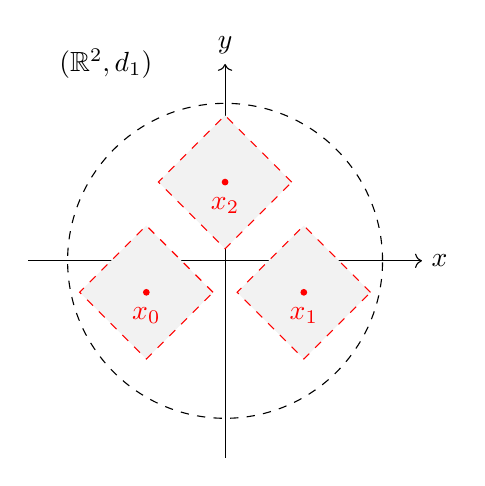
\begin{tikzpicture}
            \coordinate (x0point) at (-1, -.4);
            \coordinate (x1point) at (1, -.4);
            \coordinate (x2point) at (0, 1);
            \draw[->] (-2.5, 0) -- (2.5, 0) node[right] {$x$};
            \draw[->] (0, -2.5) -- (0, 2.5) node[above] {$y$} node[left=.8cm]
                {$ (\mathbb{R}^2, d_1) $};
            \draw[dashed] (0, 0) circle (2cm);
            \foreach \i in {0, 1, 2} {
                \node[diamond, draw, minimum width=1.7cm, minimum height=1.7cm,
                    dashed, red, fill=ballfill] at (x\i point) {};
                \filldraw[red] (x\i point) circle (1pt) node[below, yshift=-2pt]
                    {$ x_\i $};
            }
        \end{tikzpicture}
        \captionof{figure}{Considering the $ d_2 $-defined unit circle $
            \Lambda $ as an open set in the $ \left(\mathbb{R}^2, d_1\right) $
            space.}
    \end{minipage}
\end{example}
\begin{definition}{Closure}{closure}
    Let $ (X, d) $ be a metric space and $ A \subseteq X $. Then the
    \emph{closure} of $ A $, denoted by $ \overline{A} $, is defined to be $
    \overline{A} = A \cup \partial A $.

    \centering
    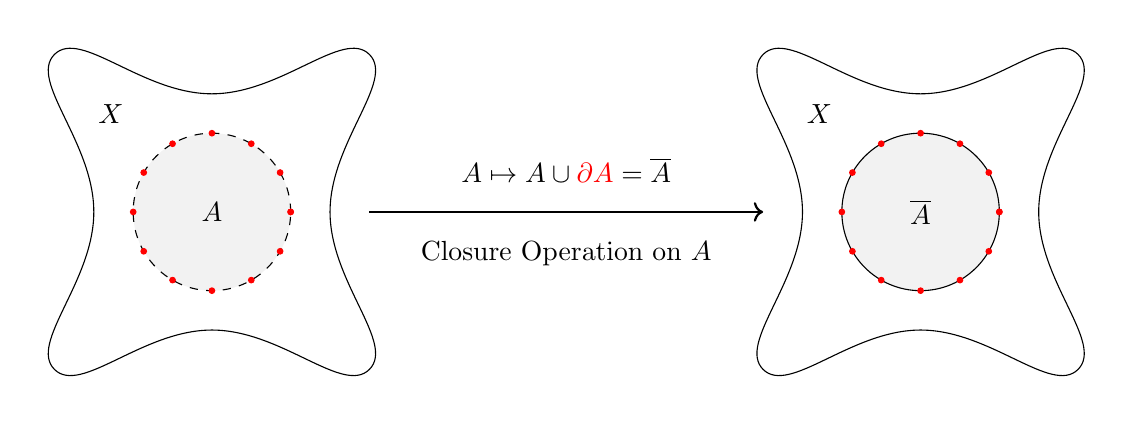
\begin{tikzpicture}
        \coordinate (leftball) at (0, 0);
        \coordinate (rightball) at (9, 0);
        \coordinate (leftbound) at (2, 0);
        \coordinate (rightbound) at (7, 0);
        \pic at (leftball) {squarespace};
        \draw[fill=ballfill, dashed] (leftball) circle[radius=1] node {$ A $}
            node [above left=1cm] {$ X $};
        \pic at (rightball) {squarespace};
        \draw[fill=ballfill] (rightball) circle[radius=1] node
            {$ \overline{A} $} node [above left=1cm] {$ X $};
        \foreach \i in {0, 30, ..., 360} {
            \filldraw[red] (leftball)++(\i:1cm) circle (1pt);
            \filldraw[red] (rightball)++(\i:1cm) circle (1pt);
        }
        \draw[->, thick] (leftbound) -- (rightbound) node [above, pos=.5,
            yshift=7pt] {$ A \mapsto A \cup {\color{red}\partial A} =
            \overline{A} $} node [below, pos=.5, yshift=-7pt]
            {Closure Operation on $ A $};
    \end{tikzpicture}
    \captionof{figure}{Encapsulating the boundary of an open set $ A $ is the
    most `efficient' way of generating a closed set $ \overline{A} $ with the
    same interior $ A^o $.}
\end{definition}
\begin{theorem}{The closure is closed}{closure-closed}
    For an open set $ A \subseteq X $, the closure $ \overline{A} $ is closed.
    \begin{proof}
        By \cref{theorem:open-subset-closed-complement}, $ \overline{A} $ is
        closed if and only if $ \left(\overline{A}\right)^c $ is open.\\
        If $\left(\overline{A}\right)^c = \emptyset $, then we are done since the
        empty set is known to be open; thus we assume that $
        \left(\overline{A}\right)^c \neq \emptyset $.
        
        To prove the openness of
        this non-empty set, we consider an arbitrary point $ x \in
        \left(\overline{A}\right)^c $ and construct an $ \epsilon > 0 $ such
        that $ B(x, \epsilon) \subseteq \left(\overline{A}\right)^c $.\\
        Take $x \in (\overline{A})^c$, then since $ \overline{A} = A \cup \partial A $, $ x \not\in A $ and $ x
        \not\in \partial A $. \\
        As $ x
        \not\in \partial A $, then $\exists \epsilon>0 $ such that  $\forall x$, $B(x, \epsilon) \subseteq A^c$ or $  B(x, \epsilon) \subseteq A$, but since $ x \not\in A $, $ B(x, \epsilon) \subseteq A^c $ is the only
        possibility.\\
        We also require that there is an $ \epsilon > 0 $ such that $ B(x, \epsilon)
        \cap \partial A = \emptyset $. By way of contradiction, suppose that
        there exists a $ y \in B(x, \epsilon) $ such that $ y \in \partial A $.
        By definition \cref{definition:boundary-points}, for all $ \delta > 0 $,
        \begin{equation}
            B(y, \delta) \cap A \neq \emptyset \text{ and } B(y, \delta) \cap
            A^c \neq \emptyset.
        \end{equation}
        If $ d(x, y) \eqcolon \epsilon^* < \epsilon $, and $ \hat{\epsilon}
        \coloneq \min\left\{ \epsilon^*, \epsilon - \epsilon^* \right\} $, then
        $ B(y, \hat{\epsilon}/2) \subseteq B(x, \epsilon) $. But $ B(y,
        \hat{\epsilon}) \cap A \neq \emptyset $. This is a contradiction: no
        such $ y $ can exist as $B(x, \epsilon)\subseteq A^c$.\\
        This shows that $ B(x, \epsilon)
        \cap \partial A = \emptyset $ and so, $\forall x \in (\overline{A})^c$ there is an $\epsilon>0$ such that $ B(x, \epsilon) \subseteq (\overline{A})^c
        $
        
        Therefore, by \cref{theorem:openness-open-balls} $, \left(\overline{A}\right)^c $ is open, and so $
        \overline{A} $ is closed.
    \end{proof}
    \centering
    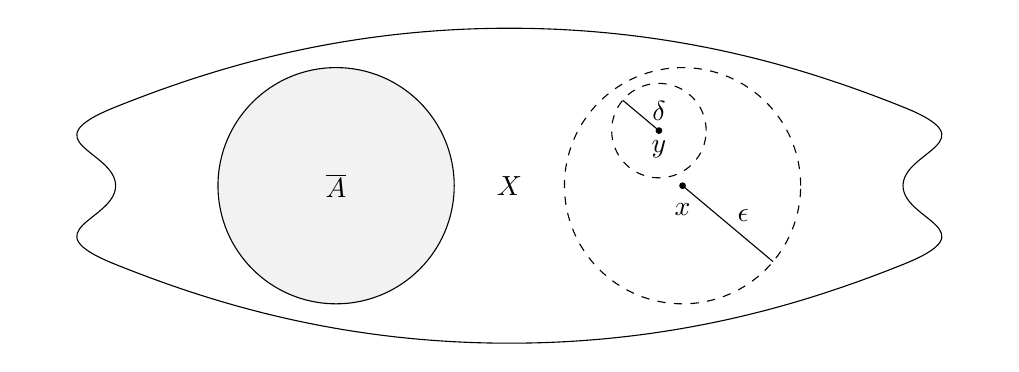
\begin{tikzpicture}
        \coordinate (apos) at (-2.2, 0);
        \coordinate (xpos) at (2.2, 0);
        \coordinate (ypos) at (1.9, .7);
        \pic at (0, 0) {longspace};
        \node at (0, 0) {$ X $};
        \draw[fill=ballfill] (apos) circle (1.5cm) node {$ \overline{A} $};
        \draw[dashed] (xpos) circle (1.5cm);
        \filldraw (xpos) circle (1pt) node[below, yshift=-3pt] {$ x $};
        \draw (xpos) -- ++(320:1.5cm) node[right, pos=.5, yshift=3pt]
            {$ \epsilon $};
        \draw[dashed] (ypos) circle (.6cm);
        \filldraw (ypos) circle (1pt) node[below] {$ y $} node[above]
            {$ \delta $};
        \draw (ypos) -- ++(140:.6cm);
    \end{tikzpicture}
    \captionof{figure}{The open ball $ B(x, \epsilon) $ lies entirely within the
        complement of the closure of $ A $, within which $ B(y, \delta) $ is
        nested.}
\end{theorem}
\pagebreak

\lecture{Lecture VII}{}{
    Lecture Seven demonstrates that a space is closed if and only if it is equal
    to its own closure, and moves to introduce the topic of
    limit/accumulation/cluster points whilst proving some useful related
    properties.
}{\DTMdisplaydate{2023}{10}{17}{Tuesday}}
\begin{theorem}{The closure of the open ball is the closed ball in \texorpdfstring{$\mathbb{R}^n$}{n-dimensional Euclidean space}}{close-open-ball}
In the metric space $(\mathbb{R}^n,d_2)$, the closure of the open ball centred at $x$ of radius $r$ is the closed ball, that is
\begin{equation}
    \overline{B(x,r)} =\overline{B}(x,r)
\end{equation}
NOTE: this is not true for all metric spaces.
\end{theorem}
\begin{theorem}{Relationships between a closed set and its closure}{closed-set-closure}
    If $ A \subseteq X $ is closed, then $ A = \overline{A} $; if $ A =
    \overline{A} $, then $ A $ is closed. That is, $ A $ is closed if and only
    if $ A = \overline{A} $.
    \begin{proof}
        \iffforward If $ A = \overline{A} $, then $ \overline{A} $ is closed by
        \cref{theorem:closure-closed}. Thus $ A $ is closed.

        \iffbackward If $ A $ is closed, then $ \partial A \subseteq A$ by
        \cref{definition:open-closed-clopen-sets}. Then, $ A = \partial A
        \cup A = \overline{A} $.
    \end{proof}
\end{theorem}
\begin{definition}{Limit/Accumulation/Cluster Points}{limit-points}
    \begin{minipage}{.6\linewidth}
        Let $ (X, d) $ be a metric space, and $ A \subseteq X $. A \emph{limit
        point} $ y \in X $ of $ A $ is an element of $ X $ for which
        \begin{equation}
            \left[ B(y, \epsilon) \setminus \{y\} \right] \cap A \neq \emptyset
            \text{ for all } \epsilon > 0.
        \end{equation}
        The \emph{derived set} of $ A $ is denoted $ A^\prime $, and is defined
        to be the set of all limit points of $ A $. Limit points are sometimes called \emph{accumulation
        points} or \emph{cluster points}.
    \end{minipage}\hfill
    \begin{minipage}{.35\linewidth}
        \centering
        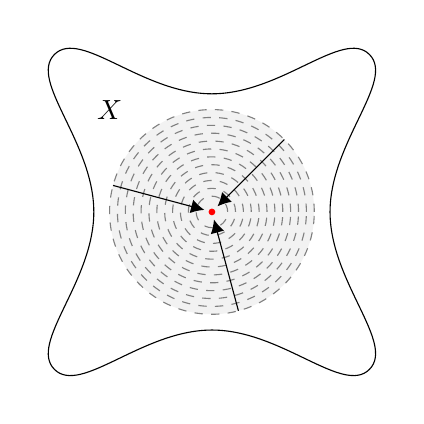
\begin{tikzpicture}
            \pic at (0, 0) {squarespace};
            \node at (-1.3, 1.3) {$ X $};
            \fill[ballfill] (0, 0) circle (1.3cm);
            \foreach \radius in {1.3, 1.2, ..., .1}
                \draw[dashed, gray] (0, 0) circle (\radius cm);
            \filldraw[red] (0, 0) circle (1pt);
            \foreach \angle in {45, 165, 285}
                \draw[-{Latex[width=5pt]}] (\angle:1.3cm) -- (\angle:.1cm);
        \end{tikzpicture}
        \captionof{figure}{As the open balls contract \emph{ad infinitum}, we
            can still find non-centroid points of $ A $.}
    \end{minipage}
\end{definition}
\begin{theorem}{A closed set contains its limit points}{closed-contains-limits}
For a closed set $F \subseteq X$, $F$ contains its limit points
\begin{proof}
    Suppose $F$ is closed and $\exists y$ such that $y \in F^\prime$ but $y \notin F$.\\
    Take $\epsilon>0$ and consider $B(y,\epsilon)$:
    \begin{itemize}
        \item[(i)] By definition of a limit point, $\exists y^\prime \neq y \in F$ such that $y^\prime \in B(y, \epsilon) \implies B(y, \epsilon) \cap F \neq \emptyset$  
        \item[(ii)]  $y \in B(y,\epsilon)$ and $y \notin F$, so $y \in F^c \implies B(y, \epsilon) \cap F^c \neq \emptyset$
    \end{itemize}
So (i) and (ii) $\implies y$ is a boundary point of $F$, and so $y \in F$ since F is closed. However, this is a contradiction and thus our assumption is incorrect and $ y \in F$.
\end{proof}
\end{theorem}
\begin{theorem}{The closure of a set is the union of the base set and its derived set}{closure-limit-union}
    For a set $ A \subseteq X $, $ \overline{A} = A \cup A^\prime $.
    \begin{proof}
        If $ A $ is closed, then the result is immediate: $ \overline{A} = A $
        (by \cref{theorem:closed-set-closure}), so $ A^\prime \subseteq A =
        \overline{A} $. Thus, we assume that $ A $ is open. If $ A^\prime =
        \emptyset $, then $ A^\prime \subseteq \overline{A} $, since $ A $ has
        no limit points; therefore, we also assume that $ A^\prime $ is non-empty. We
        will show the equality $ \overline{A} = A \cup A^\prime $ for an open
        non-empty set $ A $ through the principle of double-inclusion.

        \iffforward Without loss of generality, suppose that $ y $ is such that
        $ y \in \partial A $ and $ y \not\in A $. For any choice of $ \epsilon >
        0 $, we know that $ B(y, \epsilon) \cap A \neq \emptyset $. Since $ y
        \not\in A $, there exists a $ y^\prime \neq y \in A, B(y, \epsilon) $.
        This is consistent with \cref{definition:limit-points}. Thus, $ y $ is a
        limit point, so $ A^\prime \subseteq \overline{A} $ and $ A \cup
        A^\prime \subseteq \overline{A} $.

        \iffbackward Given that $ A $ is not closed, there exists a $ y \in
        A^\prime $ such that $ y \not\in A $. Take $ \epsilon > 0 $ and note
        that $ B(y, \epsilon) \cap A \neq \emptyset $ and $ B(y, \epsilon) \cap
        A^c \neq \emptyset $. Thus, by \cref{definition:boundary-points}, $ y $
        is a boundary point, and thus $\overline{A} \subseteq A \cup A^\prime$. 
        
        Hence, $ \overline{A} = A \cup \partial A = A \cup A^\prime $ for any
        $ A \subseteq X $.
    \end{proof}
\end{theorem}
\begin{definition}{Definitions of closed}{closed-def}
For any set $A \subseteq X$, its \emph{closeness} can be defined in many ways:
    \begin{align}
            A \text{ is closed} &\iff \partial A \subseteq A
                &&\mathrm{[\Cref{definition:open-closed-clopen-sets}]} \\
            &\iff A^c \text{ is open}
                &&\mathrm{[\Cref{theorem:open-subset-closed-complement}]}%
                \label{eqn:closure-limit-union-open} \\
            &\iff A^c \cap \partial \left( A^c \right) = \emptyset
                &&\mathrm{[\Cref{definition:open-closed-clopen-sets}]} \\
            &\iff A^c \cap \partial A = \emptyset
                &&\mathrm{[\Crefrange{eqn:boundary-complement-boundary-first}%
                    {eqn:boundary-complement-boundary-last}]} \\
            &\iff \forall x \in A^c,\, \exists \epsilon > 0 \text{ s.t. }
                B(x, \epsilon) \subseteq A^c\quad
                &&\mathrm{[\Cref{eqn:closure-limit-union-open}]} \\
            &\iff A = \overline{A} \\
            &\iff A \supseteq A^\prime
        \end{align}
\end{definition}
\begin{definition}{Topological Interpretation of Closure}{topological-closure}
    Let $ (X, d) $ be a metric space, and $ A \subseteq X $. Then,
    \begin{equation}
        \overline{A} = \bigcap_{F \in \mathcal{F}} F,
    \end{equation}
    where $ \mathcal{F} $ is the collection of all closed supersets of $ A $. This
    means that $ \overline{A} $ is the smallest closed superset of $ A $.
\end{definition}
\begin{theorem}{The closure is the smallest closed superset}{closure-smallest-superset}
For any set $A \subseteq X$, if $A \subseteq F \subseteq \overline{A}$ and $F$ is closed, then $F = \overline{A}$.
\begin{proof}
    Suppose that $y \in A^\prime$ but $y\notin F$.\\
    By definition, for any $\epsilon>0$, $B(y,\epsilon)\cap A \neq \emptyset$ and contains an $x\neq y \in A$.\\
    But $x \in A \subseteq F \implies y \in F^\prime$ but $F$ is closed so $F^\prime \subseteq F \implies y \in F$, which is a contradiction.

    Thus, $F=A \cup A^\prime = \overline{A}$
\end{proof}
\end{theorem}
\begin{definition}{Density}{density}
    Let $ (X, d) $ be a metric space and $ A \subseteq X $. Then $ A $ is said
    to be \emph{dense} in $ X $ if and only if $ \overline{A} = X $.
    Alternatively---but equivalently---for any $ x \in X $ and any $ \epsilon >
    0 $, there exists an $ a \in A $ such that $ d(x, a) < \epsilon $.
\end{definition}
\begin{example}{\texorpdfstring{$\mathbb{Q} \text{ is dense in } \mathbb{R}$}{Rationals are dense in reals}}{rational-reals}
    We can say $\mathbb{Q}$ is dense in $\mathbb{R}$ since for any $x \in \mathbb{R}$ and and $\epsilon>0$, there exists $p/q \in \mathbb{Q}$ such that $\vert x - p/q \vert < \epsilon$.

    Thus $\overline{\mathbb{Q}}=\mathbb{R}$
\end{example}
\pagebreak

\lecture{Lecture VIII}{Viewer.aspx?id=90ed9c29-e6e1-4fa4-a3a8-b0a000d532b9}{
    Lecture Eight introduces the concept of sequences in metric spaces and provides an understanding of convergence in terms of topology. It also proves that equivalent sequences have the same convergent sequences.
}{\DTMdisplaydate{2023}{10}{19}{Thursday}}
\begin{definition}{Sequences in a metric space}{seq-defn}
    A sequence in a metric space $(X,d)$ is an element $x \in X^\mathbb{N}$, where
    \begin{equation}
        x = (x_1, x_2, x_3, \dots, x_n, \dots);  x_i \in X
    \end{equation}
This sequence is denoted as $(x_n)_{n\in \mathbb{N}}$ or $(x_n)_{n=1}^{\infty}$.
\end{definition}
\begin{definition}{Convergence of a sequence in a metric space}{conv-defn}
    Let $(x_n)_{n=1}^{\infty}$ be sequence in a metric space $(X,d)$.
    
    Then $(x_n)$ converges to $x \in X$ if and only if for any $\epsilon>0$, there exists $N = N(\epsilon)>0$ such that $d(x_n, x)<\epsilon$ for all $n>N$.\\
    Equivalently, $(x_n)$ converges to $x \in X$ if and only if for any $\epsilon>0$, there exists $N = N(\epsilon)>0$ such that $x \in B(x, \epsilon)$ for all $n>N$.

    If this is the case, we write $x_n \to x$ as $n \to \infty$ and $x$ is called the limit. 
    \begin{equation}
        x_n \to x \text{ as } n \to \infty \iff d(x_n,x)\to 0 \text{ as } n \to \infty 
    \end{equation}
    If no such $x$ exists, then we say $(x_n)_{n=1}^{\infty}$ is \emph{divergent}.
\end{definition}
\begin{theorem}{Convergence in \texorpdfstring{$\mathbb{R}^k$}{k-dimensional Euclidean space} is equivalent to convergence of each sequence in \texorpdfstring{$\mathbb{R}$}{reals}}{conv-equiv}
Let $\vec{x}_n \in \mathbb{R}^k$, where $\vec{x}_n = (x_1^{(n)}, x_2^{(n)},\dots,x_k^{(n)})$. Then, 
\begin{equation}
    \begin{split}
        \vec{x}_n \to \vec{x} \iff x_i^{(n)} \to x_i \text{ as } n \to \infty \\
        \text{where }\vec{x} = (x_1, x_2,\dots,x_k)
    \end{split}
\end{equation}
\begin{proof}
    We will prove this for $(X,d_\infty)$.
\iffforward Suppose $\vec{x}_n \to \vec{x}$ as $n \to \infty$. \\
Let $\epsilon>0$ be given. Then, by \cref{theorem:conv-equiv}, there exists $N>0$ such that $d_\infty(\vec{x}_n, \vec{x})<\epsilon$ for all $n>N$. That is, $\max\limits_{1\leq i \leq k}\vert x_i^{(n)}-x_i \vert < \epsilon$ for all $n>N$, and so, $\vert x_i^{(n)}-x_i \vert < \epsilon$ for all $n>N$ and $1\leq i \leq k$.\\
But this means the real sequence $\left(x_i^{(n)}\right)^\infty_{n=1}$ converges to $x_i$.

\iffbackward Suppose for each $i \in \{1,2,\dots, k\}$, the sequence $\left(x_i^{(n)}\right)^\infty_{n=1}$ converges to $x_i$ as $n \to \infty$.\\
Let $\epsilon>0$. Then for any $i \in \{1,2,\dots, k\}$, there exists $N_i>0$ such that $\vert x_i^{(n)}-x_i \vert < \epsilon$ for all $n>N_i$.\\
Let $N\coloneqq\max\{N_1, N_2, \dots, N_k\}$. Then, $\vert x_i^{(n)}-x_i \vert < \epsilon$ for $n>N$ and each $i \in \{1,2,\dots, k\}$. This means that for $n>N$, $\vec{x}_n \to \vec{x}$.

Therefore, convergence in $\mathbb{R}^k$ is equivalent to convergence in $\mathbb{R}$ of each sequence.
\end{proof}
\end{theorem}
\begin{example}{Different metrics on same set can have different convergent sequences}{diff-metric-same-set}
    Consider the sequence $\left(f_n\right)_{n=1}^\infty \in C\left([0,1]\right)$ where 
    \begin{equation}
        \begin{split}
            f_n \colon [0,&1] \to \mathbb{R}\\
            f_n(t) &= t^n
        \end{split}
    \end{equation}
We will compare convergence in the $d_2$ metric and the $d_\infty$ metric:
\begin{itemize}
    \item[(i)] $d_2(f_n,0)$ as $n \to \infty$:
        \begin{align}
        d_2(f_n, 0) &= \left( \int^1_0\left(f_n(t)-0\right)^2\, dt\right)^{1/2}\\
        &=\left( \int^1_0\left(t^n\right)^2\, dt\right)^{1/2}\\
        &=\left( \int^1_0 t^{2n}\, dt\right)^{1/2}\\
        &=\left[\sqrt{\frac{1}{2n+1}t^{2n+1}}\right]^1_0\\
        &= \sqrt{\frac{1}{2n+1}} \to 0 \text{ as } n \to \infty
    \end{align} 
    \item[(ii)] $d_\infty(f_n,0)$ as $n \to \infty$:
        \begin{align}
            d_\infty(f_n,0) &= \sup\{\vert f_n(t) -0\vert\colon t \in [0,1]\} \\
            &= \sup\{\vert f_n(t) \vert\colon t \in [0,1]\} \\
            &= \sup\{\vert t^n \vert\colon t \in [0,1]\} \\ 
            &= 1 \,\,\, \forall n \in \mathbb{N} \not\to 0 \text{ as } n \to \infty
        \end{align}
\end{itemize}
Thus, different metrics on the same set may lead to a different convergence.
\end{example}
\begin{theorem}{Equivalent metrics have the same convergent sequences}{equiv-metric-same-conv}
    Suppose that $(X,d)$ and $(Y,\Tilde{d})$ are \emph{equivalent}(\cref{definition:topological-equivalence}), i.e. there exists $\epsilon>0$ such that 
    \begin{equation}
        \frac{1}{\lambda}\Tilde{d}(x,y)\leq d(x,y) \leq \lambda\Tilde{d}(x,y)
    \end{equation} 
    Then, $\left(x_n\right)^\infty_{n=1} \to x$ in $(X,d) \iff \left(y_n\right)^\infty_{n=1} \to y$ in $(Y,\Tilde{d})$
    \begin{proof}
        \iffforward Suppose $x_n \to x$ as $n\to \infty$ in $(X,d)$.\\
        Let $\epsilon>0$ be given. Set $\hat{\epsilon}= \epsilon/\lambda$.\\
        Then, there exists $N>0$ such that $d(x,x_n)<\hat{\epsilon} = \epsilon/\lambda$ for all $n>N$.\\
        But $\frac{1}{\lambda}\Tilde{d}(x,y)\leq d(x,y)< \epsilon/\lambda$.\\
        Therefore, $\Tilde{d}(y_n, y) \leq \lambda d(x_n, x) \leq \epsilon$ and so $\left(y_n\right)^\infty_{n=1} \to y$ in $(Y,\Tilde{d})$.
        
        \iffbackward Can be proved analogously for $\Tilde{d}$.
    \end{proof}
\end{theorem}
\pagebreak


\lecture{Lecture IX}{Viewer.aspx?id=0fa218ae-7c44-465c-b963-b09f009bd3ea}{
    Lecture Nine introduces the uniqueness of a limit for a given sequence, the definition for point-wise convergence along with Cauchy and complete sequences. It also provides a topological definition for continuous functions.
}{\DTMdisplaydate{2023}{10}{24}{Tuesday}}
\begin{theorem}{The limit of a convergent sequence is unique}{limit-unique}
    Let $(X,d)$ be a metric and a sequence $x_n$ in $X$. If $x_n \to x$ and $x_n \to y$ then $x=y$. We write
    \begin{equation}
        \lim_{n\to \infty} x_n = x
    \end{equation}
    \begin{proof}
        Assume $x\neq y$, then $d(x,y) = \epsilon >0$.\\
        Set $\delta=\epsilon/2$.\\
        As $x_n \to x$  as $n \to \infty$ then, by \cref{theorem:conv-equiv}, there exists $N = N(\delta) > 0$ such that $d(x_n, x) < \delta = \epsilon/2$ for all $n>N$. Also, there exists $\hat{N} = N(\delta) > 0$ such that $d(x_n, y) < \delta = \epsilon/2$ for all $n>\hat{N}$.\\
        Set $M = \max\{N, \hat{N}\}$, then both the above conditions should be held for all $n>M$.

        Using the triangle inequality, for all $n>M$, 
        \begin{align}
            d(x,y) &\leq d(x, x_n) + d(x_n, y)\\
            &< \delta + \delta\\
            &= \epsilon
        \end{align}
        But $d(x,y)=\epsilon$ and so it is a contradiction.

        Therefore, the assumption was incorrect and $x=y$.
    \end{proof}
\end{theorem}
\begin{definition}{Series in \texorpdfstring{$(\mathbb{R},d)$}{the real space}}{series-defn}
    The series of a sequence $ x_n \in \mathbb{R} $ is defined to be the limit (if it exists) of the \emph{partial sum sequence} $S_k$ as $k \to \infty$, where 
    \begin{equation}
        S_k = \sum_{n=1}^k x_n
    \end{equation}
    The series is denoted as $S_\infty$, where 
    \begin{equation}
        S_\infty \coloneqq \lim_{k\to\infty} S_k
    \end{equation}

    This can be moved to an abstract setting if $(X,d)$ has a notion of addition.
\end{definition}
\begin{definition}{Point-wise convergence of a sequence of functions}{pointwise-conv}
    Let $\left(f_n\right)^\infty_{n=1}$ be a metric sequence of function, where 
    \begin{equation}
        f_n \colon X \to Y
    \end{equation}
    The function $f$ is the point-wise limit of $\left(f_n\right)^\infty_{n=1} \iff$ for any $x_0 \in X$, $\lim\limits_{n \to\infty} f_n(x_0) = f(x_0)$.

    Thus, $f_n$ converges to $f$ point-wise:
    \begin{equation}
        f_n \xrightarrow{\text{p.t.}} f \, \text{as } n\to \infty
    \end{equation}
    
\end{definition}
\begin{definition}{Continuity of functions in a metric space}{continuity-defn}
    Let $f: X\to Y$ be a function from $(X,d)$ to $(Y,\hat{d})$.
    \begin{itemize}
        \item[\textbf{\emph{Local}}] $f$ is continuous at $x_0 \in X \iff f(x_n) \to f(x_0)$ whenever the sequence $(x_n)^\infty_{n=1} \to x_0$. 
        \item[\textbf{\emph{Global}}] $f$ is continuous $\iff f$ is continuous at every $x_0 \in X$ 
    \end{itemize}
    We can generalise $C([0,1])$ to $C(X,Y) = \{f:X\to Y \, \vert \,f \text{ is continuous}\}$
\end{definition}
\begin{definition}{Cauchy sequence}{cauchy-defn}
    Let $\left(x_N\right)^\infty_{n=1}$ be a sequence.
    
    Then $x_n$ is \emph{cauchy} if and only if, for any $\epsilon>0$, there exists $N>0$ such that $d(x_n, x_m)<\epsilon$ for all $n, m>N$.
\end{definition}
\begin{theorem}{Convergence implies Cauchy}{conv-implies-cauchy}
    Let $(X,d)$ be a metric space and $\left(x_n\right)^\infty_{n=1}$ be a convergent sequence to $x \in X$. Then $\left(x_n\right)^\infty_{n=1}$ is Cauchy.
    \begin{proof}
        Let $\epsilon>0$ be given.\\
        Set $\delta = \epsilon/2 >0 $.\\
        Then, by \cref{definition:conv-defn}, there exists $N = N(\delta) > 0$ such that $d(x_n,x)<\delta$ for all $n>N$. But for all $n,m > N$, using the triangle inequality, it holds that
        \begin{align}
            d(x_n,x_m) &\leq d(x_n, x) + d(x, x_m)\\
            &< \delta+\delta\\
            &= \epsilon
        \end{align}
        Thus, by \cref{definition:cauchy-defn}, $\left(x_n\right)^\infty_{n=1}$ is Cauchy.

        Therefore, convergence implies Cauchy.
    \end{proof}
\end{theorem}
\begin{example}{Cauchy does not imply convergence}{cauchy-notimply-conv}
    Let $(X,d)$ be a metric space where $X = (0, \infty)$, and let $x_n = \frac{1}{n}$.

    $x_n \to 0$ as $n \to \infty$, however, $0\notin X$ so the sequence is not convergent in $X$.
\end{example}
\pagebreak

\lecture{Lecture X}{Viewer.aspx?id=1358f782-4f58-49d2-b236-b0a700ef3a9f}{
    Lecture Ten begins with the idea of a sequence tending to infinity, along with a few more properties of Cauchy with examples, as well as introduces the notion of a sub-sequence. It then goes onto define completeness in a sequence along with its properties and application to the Euclidean space.
}{\DTMdisplaydate{2023}{10}{26}{Thursday}}
\begin{theorem}{Limit of a sequence to infinity}{inf-limit}
    A sequence $x_n$ tends to $\infty \iff$ for any $M>0$, there exists $N>0$ such that $M<x_n$ for all $n>N$
\end{theorem}
\begin{theorem}{Not Cauchy implies not convergent}{contrapositive-cauchy}
    For any sequence $\left(x_n\right)^\infty_{n=1}$, if $(x_n)$ is not Cauchy, it is not convergent.
    \begin{proof}
        Taking the contrapositive of \cref{theorem:conv-implies-cauchy}, we get that \emph{not Cauchy} $\implies$ \emph{not convergent}.
    \end{proof}
\end{theorem}
\begin{example}{The harmonic series is divergent}{harmonic-divergent}
    Given the metric space $(\mathbb{R},d)$, the \emph{harmonic series} $S_\infty$ is defined as 
    \begin{equation}
        S_\infty = \sum_{n=1}^\infty \frac{1}{n}
    \end{equation}
    By \cref{definition:series-defn}, $S_\infty \coloneqq \lim\limits_{N\to \infty}S_N$. We can show $\left(S_N\right)^\infty_{N=1}$ is not convergent by showing $\left(S_N\right)^\infty_{N=1}$  is not Cauchy.

    Consider
    \begin{align}
        \begin{split}
            S_{2N}-S_N ={}&\left(\dfrac{1}{2N}+\dfrac{1}{2N-1}+\dfrac{1}{2N-2}+\dots+\dfrac{1}{N+1}+\dfrac{1}{N}+\dfrac{1}{N-1}+\dots+1\right)-\\
            &\left(\dfrac{1}{N}+\dfrac{1}{N-1}+\dots+1\right)
        \end{split}\\
            ={}& \left(\dfrac{1}{2N}+\dfrac{1}{2N-1}+\dfrac{1}{2N-2}+\dots+\dfrac{1}{N+1}\right)\\
            \geq{}& \dfrac{1}{2N}\cdot N\\
            ={}& \dfrac{1}{2}
    \end{align}
    By the definition of Cauchy, given $\epsilon>0$, we would need to find $K>0$ such that $\vert S_M - S_N \vert <\epsilon$ for all $M, N >K$. However, if $M\geq2N$ then $\vert S_M - S_N \vert \geq 1/2$, so the sequence is not Cauchy.

    Therefore, by \cref{theorem:contrapositive-cauchy}, $\left(S_N\right)^\infty_{N=1}$ is not convergent i.e. divergent.
\end{example}
\begin{definition}{Sub-sequences}{subsequences-defn}
    Given $(X,d)$ and a sequence $(x_n)_{n=1}^\infty$ in $X$.

    A sub-sequence of $(x_n)$ is a sequence of elements $x_n, x_{n_2}, x_{n_3},\dots, x_{n_k},\dots$ where $n_i \in \mathbb{N}$ and $n_1<n_2<n_3<\dots<n_k<\dots$ ($n_k \to \infty$ as $k\to \infty$)
\end{definition}
\begin{definition}{Divergence in sub-sequences}{subsequences-div}
    Let $\left(x_n\right)^\infty_{n=1}$ be a sequence in $X$.

    If there exists $n_1<n_2<\dots<n_k<\dots$ and $n_1^\prime<n_2^\prime<\dots<n_k^\prime<\dots$ such that $x_{n_i}\to\infty$ as $i \to \infty$ and $x_{n^\prime_i}\to\infty$ as $i \to \infty$ and $x\neq y$, then $\left(x_n\right)^\infty_{n=1}$ is divergent.
\end{definition}
\begin{theorem}{Convergence in sub-sequences}{subsequences-conv}
    Let $(X,d)$ be a metric space, $\left(x_n\right)^\infty_{n=1}$ be a Cauchy sequence and $\left(x_{n_k}\right)^\infty_{n=1}$ a convergent sub-sequence.
    
    Then, $\left(x_n\right)^\infty_{n=1}$ is convergent and $\lim\limits_{n\to\infty}x_n = \lim\limits_{k\to\infty}x_{n_k}=x$
    \begin{proof}
        By \cref{definition:conv-defn}It is sufficient to show that for any $\epsilon>0$, there exists $N>0$ such that $d(x_n,x)<\epsilon$ for all $n>N$. 

        Let $\epsilon>0 be given$. \\
        By definition of Cauchy, we can find $N_1>0$ such that $d(x_n,x_m)<\epsilon/2$ for an $n, m>N_1$.\\
        By definition of convergence, we can find $N_2>0$ such that $d(x_{n_k},x)<\epsilon/2$ for an $k>N_2$.\\
        Choose $N=\max{N_1, N_2}$. Thus both conditions hold for all $n,m,k>N$. It follows that 
        \begin{align}
            d(x_n,x) &\leq d(x_n, x_{n_k}) + d(x_{n_k},x_x)\\
            &< \epsilon/2 +\epsilon/2\\
            &= \epsilon
        \end{align}
    Thus, there exists $N>0$ such that $d(x_n, x) <\epsilon$ for all $n>N$. 
    \end{proof}
\end{theorem}
\begin{definition}{Complete metric space}{comp-defn}
    Let $(X,d)$ be a complete metric space.

    Then $X$ is complete $\iff$ any Cauchy sequence in $X$ converges to a point in $X$

    Equivalently, if $X$ is known to be complete and the sequence $(x_n)$ is known to be Cauchy, then there exists $x\in X$ such that $x_n\to x$ as $n \to\infty$.

    The real space $\mathbb{R}$ is known to be complete.
\end{definition}
\begin{theorem}{Completion of a metric space}{completion}
    Let $(X,d)$ be a metric space.

    Then there is a metric space $(X^*, \hat{d})$ and an isometry $\psi : X \to X^*$ such that:
    \begin{itemize}
        \item[i)]$X^*$ is complete
        \item[ii)]$\overline{\psi(x)} = X^*$ 
    \end{itemize}
    $X^*$ is called the \emph{completion} of $X$ and further, all completions of $X$ are isometric to $X^*$.
\end{theorem}
\begin{theorem}{Completing a metric space}{complete-space}
    Let $(X,d)$ be a metric space.

    If $X$ is complete, then $X^*=X$ and $\phi(x)= X$.

    If $X$ is not complete:
        \begin{itemize}
            \item Form the set $\mathcal{C}(X)$ of all possible Cauchy sequences in $X$. $\mathcal{C}(X) \neq  \emptyset$ as $(x,x,x,\dots)$ is a Cauchy sequence.
            
            \item Define an \emph{equivalence relation} $\sim$ on $\mathcal{C}(X)$ by saying
            \begin{equation}
                (x_n)\sim(y_n)\iff d(x_n, y_n)\to 0 \text{ as } n \to \infty
            \end{equation}
            
            \item Construct the set of all equivalence classes under this relation; $\mathcal{C}(X)/\sim$. An element of $\mathcal{C}(X)/\sim$ follows
                \begin{equation}
                    [(x_n)] = \{(y_n)\,\vert\, (x_n)\sim (y_n)\}
                \end{equation}

            \item Extend the metric $d$ on $X$ to a metric $\hat{d}$ on $\mathcal{C}(X)/\sim$ by setting 
            \begin{equation}
                \hat{d}\left([(x_n)],[(y_n)]\right) = \lim\limits_{n\to\infty} d(x_n, y_n)
            \end{equation}
            and show that $\hat{d}$ is a metric and well-defined.

            \item Define $\phi(x) = [\left(x\right)^\infty_{n=1}] = (x,x,x,\dots) \in \mathcal{C}(X)/\sim$ and prove that $\psi(x)$ is an isometry.

            \item Show that $\overline{\phi(X)} = \mathcal{C}(X)/\sim$ = $X^*$

            \item Show that any Cauchy sequence in $\mathcal{C}(X)/\sim$ converges to a limit in the space $\mathcal{C}(X)/\sim$. A Cauchy sequence in the space is of the form 
            \begin{equation}
            \left(\left[\left(x_n^{(1)}\right)\right],\left[\left(x_n^{(2)}\right)\right],\left[\left(x_n^{(3)}\right)\right],\left[\left(x_n^{(4)}\right)\right],\dots\right)
            \end{equation}

            \item Show uniqueness of the limit
        \end{itemize}
    \begin{proof}
        The proof can be found in Section (1.5) of Sriv
        Srirali and Vasudeva 
    \end{proof}
\end{theorem}
\pagebreak


\lecture{Lecture XI}{Viewer.aspx?id=227c74d2-ed70-4345-bed6-b0ad00abd4d4}{
    Lecture Eleven begins with a simple proof to show the k-dimensional Euclidean space is complete, followed by a generalisation of the first of three C's of metric spaces: continuity, using $\epsilon$-$\delta$. It then ends with the discussion and proof for 5 definitions of continuity.
}{\DTMdisplaydate{2023}{11}{7}{Tuesday}}
\begin{example}{Steps to show (non/)completeness}{check-complete}
    To show a space is not complete requires finding one Cauchy sequence that \emph{converges} to a point not in the space.

    To show a space is complete:
    \begin{itemize}
        \item Start with an arbitrary Cauchy sequence $(x_n)_{n=1}^\infty$
        \item Construct a candidate limit $x$
        \item Show that $x \in X$
        \item Show that $\lim_{n\to\infty}x_n=x$
    \end{itemize}
    This can be demonstrated by showing the metric space $(\mathbb{R}^k, d_\infty)$ is complete.

    \begin{proof}
        Take a Cauchy sequence $(\vec{x}_n)_{n=1}^\infty \in \mathbb{R}^k$. Recall notation: $\vec{x}_n=(x_n^{(1)},x_n^{(2)},x_n^{(2)}, \dots,x_n^{(k)})$. We know that the sequence is Cauchy implies that, given $\epsilon>0$, there exists $N>0$ such that $d_\infty(\vec{x}_n, \vec{x}_m)<\epsilon$ for all $n,m>N$. 

        So $\max\{\vert\vec{x}_n^{(i)}-\vec{x}_m^{(i)}\vert\}<\epsilon$ for all $n,m>N$. 

        Therefore, each real sequence $(x_n^{(i)})_{n=1}^\infty$ is Cauchy. But $\mathbb{R}$ is complete and there exists $x_i$ such that $\lim_{n\to\infty}x_n^{(i)} = x_i$:
        \begin{align*}
            \left(x_1^{(1)},x_1^{(2)},\dots,x_1^{(k)}\right) &= \vec{x}_1\\
            \left(x_2^{(1)},x_2^{(2)},\dots,x_2^{(k)}\right) &= \vec{x}_2\\
            \left(x_3^{(1)},x_3^{(2)},\dots,x_3^{(k)}\right) &= \vec{x}_3\\
            &\shortvdotswithin{=}\notag
            \left(x_n^{(1)},x_n^{(2)},\dots,x_n^{(k)}\right) &= \vec{x}_n\\
            &\shortvdotswithin{=}\notag 
        \end{align*}
        Thus, the sequence $(\vec{x}_n)^\infty_{n=1}$ converges to $\vec{x}=(x_1,x_2,x_3, \dots, x_k) \iff \left(x_n^{(i)}\right)^\infty_{n=1}$ converges to $x_i$.

        Thus, $(\vec{x}_n) \in (\mathbb{R})^\mathbb{N}$ is convergent to $(\vec{x})\in \mathbb{R}^k$  and so $(\mathbb{R}^k, d_\infty)$ is complete.
    \end{proof}
\end{example}
\begin{definition}{The $\epsilon$-$\delta$ definition of continuity}{eps-del-defn}
    Let $f: X\to Y$ be a function from $(X,d)$ to $(Y,\hat{d})$.
    
    $f$ is continuous at $x_0 \in X \iff$ for any $\epsilon>0$, there exists $\delta>0$ such that $\hat{d}(f(x), f(x_0))<\epsilon$ whenever $d(x,x_0)<\delta$. 
\end{definition}
\begin{definition}{The $\epsilon$-$\delta$ ball definition of continuity}{eps-del-ball-defn}
    Let $f: X\to Y$ be a function from $(X,d)$ to $(Y,\hat{d})$.

    $f$ is continuous at $x_0 \in X \iff$ for any $\epsilon>0$, there exists $\delta>0$ such that $f(B(x_0,\delta))\subseteq B(f(x_0,\epsilon))$ 

    \begin{proof}
        From \cref{definition:eps-del-defn}, we find that $d(x,x_0)<\delta$ is equivalent to creating an open ball around $x_0$ of length $\delta$: $B(x_0,\delta)$. 
        
        If $f$ is continuous, then for all points $x \in B(x_0,\delta)$, it is true that $\hat{d}(f(x_0),f(x))<\epsilon$. This, similarly, is equivalent to creating an open ball around $f(x_0)$ of length $\epsilon$: $B(f(x_0), \epsilon)$.

        Therefore, $f(B(x_0,\delta))\subseteq B(f(x_0,\epsilon))$.
    \end{proof}
    
    
\end{definition}
\begin{definition}{The open set definition of continuity}{open-set-defn}
    Let $f: X\to Y$ be a function from $(X,d)$ to $(Y,\hat{d})$.

    $f$ is continuous at $x_0 \in X \iff$ for any open set $V \subseteq Y$ with $f(x_0)\in V$, there exists an open ball $B \subseteq X$ with $x_0 \in B$ and $f(B)\subseteq V$.

    \begin{proof}
        Let $V$ be open in Y. By \cref{open-def}, there exists $\epsilon>0$ such that $B(y, \epsilon)\subseteq V$ for all $y \in V$, where $y=f(x_0)$.

        From \cref{definition:eps-del-ball-defn}, we know there exists an open ball $B(x_0, \delta)$ such that $f(B) \subseteq B(f(x_0),\epsilon) = V$.
    \end{proof}
    
\end{definition}
\begin{definition}{Topological definition of continuity}{cont-topological-defn}
    Let $f: X\to Y$ be a function from $(X,d)$ to $(Y,\hat{d})$.
    
    $f$ is continuous at $x_0 \in X \iff$ for any open set $V \subseteq Y$, there exists an open set $U \subseteq X$ with $x_0 \in U$ and $f(U)\subseteq V$.
    \begin{proof}
        We can derive this from \cref{definition:open-set-defn} by replacing the open ball with an open set.
    \end{proof}
\end{definition}
\begin{definition}{Sequential definition of continuity}{cont-seq-defn}
    Let $f: X\to Y$ be a function from $(X,d)$ to $(Y,\hat{d})$.
    
    $f$ is continuous at $x_0 \in X \iff$ for any sequence $x_n$,  $\lim\limits_{n \to \infty}f(x_n) = f(x_0) $ whenever $\lim\limits_{n \to \infty}x_n = x_0$
\end{definition}
\begin{theorem}{All 5 definitions of continuity are equivalent}{cont-defn-equiv}
\begin{equation}
        \begin{split}
        \text{\cref{definition:eps-del-defn}} \implies \text{\cref{definition:eps-del-ball-defn}} \implies \text{\cref{definition:open-set-defn}} \implies\\
        \text{\cref{definition:cont-topological-defn}}\implies \text{\cref{definition:cont-seq-defn}}\implies \text{\cref{definition:eps-del-defn}}
    \end{split}
    \end{equation}
    We have already shown \cref{definition:eps-del-defn} $\implies$ \cref{definition:eps-del-ball-defn} $\implies$ \cref{definition:open-set-defn} $\implies$ \cref{definition:cont-topological-defn} in their respective definitions.
    We now need to show \cref{definition:cont-topological-defn}$\implies$\cref{definition:cont-seq-defn} and \cref{definition:cont-seq-defn}$\implies$ \cref{definition:eps-del-defn}
    \begin{proof}
        \textbf{\cref{definition:cont-topological-defn}$\implies$\cref{definition:cont-seq-defn}}:

        Let $x_0\in X$ and $(x_n)^\infty_{n=1}$, a sequence in $X$ such that $x_n \to x_0$ as $n \to \infty$.

        Assuming \cref{definition:cont-topological-defn} is true, it is sufficient to show that $f(x_n)\to f(x_0)$ as $n \to \infty$. 
        
        Let $V$ be open in $Y$ and $f(x_0)\in V$. By \cref{definition:cont-topological-defn}, there exists an open set $U \subseteq X$ such that $x_0 \in U$ and $f(U)\subseteq V$. But $U$ is open and hence there exists an $\epsilon >0$ such that $B(x_0, \epsilon)\subseteq U$.

        As $x_n \to x_0$, we can find $N>0$ such that $d(x_n, x_0)<\epsilon$ for all $n>N$. This is equivalent to $x_n \in B(x_0, \epsilon)$ for all $n>N$.

        Thus, $f(x_n)\in f(U) \subseteq V$ for all $n>N$ which is equivalent to $f(x_n) \in f(B(x_0,\epsilon))\subseteq B(f(x_0),\epsilon)$, which implies $d(f(x_n),f(x_0))<\epsilon$ for all $n>N$. 
        
        Therefore, by \cref{definition:conv-defn}, $f(x_n)\to f(x_0)$ as $n \to \infty$ and so \cref{definition:cont-topological-defn}$\implies$\cref{definition:cont-seq-defn} holds.

        \textbf{\cref{definition:cont-seq-defn}$\implies$ \cref{definition:eps-del-defn}} 

        Using contrapositive: $\neg$\cref{definition:eps-del-defn}$\implies\neg$\cref{definition:cont-seq-defn}

        ($\neg$\cref{definition:eps-del-defn}): There exists $\epsilon>0$ such that for all $\delta>0$, we have $\hat{d}(f(x),f(x_0))\geq\epsilon$ for some $x \in X$, which satisfies  $d(x,x_0)<\delta$.

        ($\neg$\cref{definition:eps-del-defn}): For any sequence $x_n$, $f(x_n) \not\to f(x_0)$ whenever $x_n \to x_0$ as $n \to\infty$

        For each $n \in \mathbb{N}$ we define the set:
        \begin{equation}
            A_n = \{ x^\prime \in X : d(x', x_0) < 1/n \text{ and } \hat{d}(f(x^\prime),f(x_0))\geq\epsilon\}
        \end{equation}
        From above, this set is non-empty. Pick an element $x_n$ from $A_n$.\\
        Then $x_n \to x$ as $n \to \infty$ (since $d(x_n,x)<1/n)$.\\
        But, $\hat{d}(f(x),f(x_0))\geq\epsilon>0$ so $f(x_n) \not\to f(x)$ as $n \to \infty$, which establishes $\neg$\cref{definition:cont-seq-defn}.

        Therefore, $\neg$\cref{definition:eps-del-defn}$\implies\neg$\cref{definition:cont-seq-defn}  and so \cref{definition:cont-seq-defn}$\implies$ \cref{definition:eps-del-defn} holds.
    \end{proof}
\end{theorem}
\pagebreak

\lecture{Lecture XII}{Viewer.aspx?id=67becd92-a94f-4318-a4ae-b0af00ac252a}{
    Lecture Twelve continues to discuss continuity, while formally defining global continuity in multiple ways. It then discusses the open set characteristic of continuity, and finishes by discussing the set of continuous and bounded functions.
}{\DTMdisplaydate{2023}{11}{9}{Thursday}}
\begin{definition}{Topological definition of global continuity}{global-cont-topological-defn}
   Let $f: X\to Y$ be a function from $(X,d)$ to $(Y,\hat{d})$.
    
    $f$ is continuous at \emph{all} $x \in X \iff$ for any open set $V \subseteq Y$, the set $f^{-1}(V)\subseteq X$ is open.

    Equivalently, 
    \begin{align}
        f \text{ is continuous at \emph{all} } x \in X &\iff f^{-1}(V)\in T_d \text{ whenever } V \in T_{\hat{d}}\\
        &\iff f^{-1}(F) \text{ is closed whenever } F \text{ is closed} 
    \end{align}

    \begin{proof}
        Take an open set $V \subseteq Y$. For any point $y \in V$:
        
        If $V = \emptyset$ then $f^{-1}(V)=\emptyset$ and we are done.

        If $y \not\in f(x)$ then the set of points $x$ such that $f(x)=y$: $F_y = \emptyset$, so $f^{-1}(V)=\emptyset$ and we are done. 

        If $F_y \neq \emptyset$ then there exists $x \in X$ such that $f(x) = y$.\\
        Then by assumption that $V$ is open and that $f$ is continuous, there exists an open ball $B \subseteq X$ such that $ x\in B$ and $F(B) \subseteq V$.\\
        So 
        \begin{equation}
            f^{-1}(V) = \bigcup\limits_{y\in V} F_y  = \bigcup\limits_{x\in f^{-1}(V)}B_x
        \end{equation}
    By \cref{theorem:topology-open-balls}, $\bigcup B_x = f^{-1}(V)$ is an element of the topology $T_d$. 
    \end{proof}
\end{definition}
\begin{theorem}{Continuity is transitive}{cont-transitive}
    Let $X, Y, Z$ be metric spaces and $f: X\to Y$ be continuous and $g: Y \to Z$ be continuous. Then $g \circ f : X \to Z$ is continuous.
    \begin{proof}
        Let $V \subseteq Z$ be open. Then $g^{-1}(V) \subseteq Y$ is open $\implies f^{-1}(g^{-1}(V))$ is open in $X$

        As $(g\circ f)^{-1}(V) = f^{-1}(g^{-1}(V))$ is open, it follows that $(g\circ f)$ is continuous by \cref{definition:global-cont-topological-defn}.
    \end{proof}
    (Note: a composition can be continuous but $f$ or $g$ not)  
\end{theorem}
\begin{theorem}{A function mapping a point to a set of functions is continuous}{function-mapping-set}
    Let $f_1, f_2, \dots, f_k$ be continuous functions from $(X,d)$ to $(\mathbb{R}^k,d)$.

    Then $F: X \to \mathbb{R}^k$, where $F(x) = (f_1(x), f_2(x), \dots, f_k(x))$ is continuous.
    \begin{proof}
        Suppose that $x_n$ is a sequence in $X$ and $x_n \to x$ as $n \to \infty$.

        As $f_i$ is continuous, by \cref{definition:cont-seq-defn}, we know that $f_i(x_n)\to f_i(x)$ as $n \to \infty$.\\
        Recall from \cref{example:check-complete}, the sequence 
        \begin{equation}
            F(x_n) \to F(x) \text{ where } F(x) = (f_1(x),f_2(x),\dots,f_k(x))
        \end{equation}
        Therefore, by \cref{definition:cont-seq-defn}, since $F(x_n)\to F(x)$ as $n \to \infty$, the function $F$ is continuous.
    \end{proof}
\end{theorem}
\begin{theorem}{\texorpdfstring{$C([0,1])$}{The set of continuous functions} can be generalised to any metric}{generalise-set-continuous}
    Given $(X,d)$ and $(Y,\hat{d})$, the set of continuous and bounded functions $\mathscr{C}$ with the sup-metric $d_\infty$: $(\mathscr{C}(X,Y),d_\infty)$ is a metric sub-space.
    \begin{proof}
        Start with $C([0,1])$. We cannot use $d_1$ and $d_2$ as they induce notions of integration, which cannot be generalised to other metrics. We must therefore use the sup-metric $d_\infty$ as it uses the concept of a supremum.
        \begin{equation}
            d_\infty(f,g)=\sup\{\vert f(x)-g(x)\vert :  x \in X\} 
        \end{equation}
        We then pair the set $C(X,Y)$ with $d_\infty$. However, since $Y$ is paired with the metric $\hat{d}$, we have to modify $d_\infty$ accordingly:
        \begin{equation}
            d_\infty(f,g)=\sup\{\hat{d}(f(x),g(x))\, \vert \, x \in X\} 
        \end{equation}
        The problem here is since the range of $\hat{d}$ is $[0, \infty)$, there is no guarantee that such an upper bound will exist. It is therefore insufficient to only use the set of continuous functions.\\

        Consider the set of bounded functions. Let $f:X \to Y$.
        \begin{align}
            f \text{ is bounded} &\iff \text{there exists an open ball } B \subseteq Y \text{ such that } f(x)\in B \text{ for all } x \in X\\
            &\iff \text{there exists a } z \in Y \text{ and } M \in [0,\infty) \text{ such that } f(x)\in B(z,M) \text{ for all } x \in X\\
            &\iff 
        \end{align}
        The set of bounded functions can be denoted as $B(X,Y)$, and the set of all continuous and bounded functions $\mathscr{C}$, where
        \begin{equation}
            \mathscr{C}(X,Y) = B(X,Y) \cap C(X,Y)
        \end{equation}
        Therefore, $(\mathscr{C}(X,Y),d_\infty)$ is a metric sub-space.
    \end{proof}
\end{theorem}
\pagebreak

\lecture{Lecture XIII}{Viewer.aspx?id=fd3b00e1-b523-45ef-bab5-b0b400ac5f0b}{
    Lecture Thirteen continues looking at the set of continuous functions, and using this to define a stronger notion of uniform convergence. It then goes on to introduce contractions and the Contraction Mapping Theorem.
}{\DTMdisplaydate{2023}{11}{14}{Tuesday}}
\begin{definition}{A stronger notion of convergence: uniform convergence}{unif-conv}
    Consider the metric space $\mathscr{C}(X,\mathbb{K})$ where $\mathbb{K} = \mathbb{R}$ or $\mathbb{C}$ equipped with the $d_\infty$ metric.

    Let $(f_n)_{n=1}^\infty$ be a sequence from $(\mathscr{C},d_\infty)$.

    So $f_n \to f$ as $n \to \infty \iff$ for any $\epsilon>0$, there exists $N>0$ such that $d_\infty(f_n,f)<\epsilon$ for all $n>N$.

    As $d_\infty(f_n,f)=\sup\{\vert f_n(x) - f(x)\vert : x \in X\} < \epsilon$, $\vert f_n(x) - f(x)\vert$ is independent of $x$ and is always less than $\epsilon$ for all $n>N$, $x \in X$. This is \emph{uniform convergence}.

    Contrast this with \emph{point-wise convergence}: Take $x \in X$ and fix it. Consider the sequence $f_n(x) \in \mathbb{K}^\mathbb{N}$.
    $f_n \to f$ point-wise $\iff$ $f_n(x) \to f(x)$ as $n\to\infty$ for any $x \in X$. This is dependent on both $\epsilon$ and $x$, unlike \emph{uniform convergence}. 

    So, uniform convergence $\implies$ point-wise convergence, but point-wise convergence $\not\implies$ uniform convergence
\end{definition}
\begin{example}{Point-wise does not imply uniform}{pointwise-not-unif}
    Take a sequence $f_n$ from $C([0,1])$, where $f_n(t) =t^n$.

    \emph{Point-wise.} Take a fixed $t$. Then, $f_n(t) \to 0$ as $n \to \infty$. Therefore it is point-wise convergent.

    \emph{Uniform.} Take $d_\infty$. $d_\infty(f_n,f)=\sup\{|t^n-0|\}=\sup\{|t^n|\} = 1 \not< \epsilon$. Therefore, it is not point-wise convergent.
\end{example}
\begin{definition}{Fixed points}{fixed-point-defn}
    Let $f:X\to X$ be a function and $(X,d)$ a metric space. A \emph{fixed point} of $f$ is a point $y\in X$ such that $y=f(y)$.
\end{definition}
\begin{definition}{Lipschitz function}{lipschitz-defn}
    Let $f:X\to X$ be a function from the metric space $(X,d)$ to the metric space $(Y,\hat{d})$. Then $f$ is \emph{Lipschitz} if and only if, for all $x, x^\prime \in X$,
    \begin{equation}
        \hat{d}(f(x),f(x^\prime)) \leq \lambda d(x,x^\prime)
    \end{equation}
    for some $\lambda\in[0,\infty)$. The quantity $\lambda$ is known as the \emph{Lipschitz factor}. A \emph{strict contraction} is a Lipschitz function in $[0,1)$.
\end{definition}
\begin{definition}{Contraction Mapping Theorem}{cmt-defn}
    Let $(X,d)$ be a \emph{complete} metric space and $f:X \to X$ a \emph{contraction mapping}. Then $f$ has a unique fixed point, say $y \in X$ and further, a sequence $(x_n)^\infty_{n=1}$ where 
    \begin{equation}
        x_n = f(x_{n-1})
    \end{equation}
    converges to $y$. That is, $x_n \to y$ as $n \to \infty$.

    Every contraction mapping is \emph{Lipschitz continuous} and therefore uniform continuous.
\end{definition}
\pagebreak

\lecture{Lecture XIV}{Viewer.aspx?id=2f835cff-32fb-409b-9aa9-b0b600ac611b&query=16\%2F11}{
    Lecture Fourteen begins with a proof for the Continuous Mapping Theorem, encompassing most concepts we have learnt thus far. It then explains the use of the Mean Value Theorem in proving the CMT, followed by an example using the Fredholm equations snd a subsequent proof showing completeness of the set of continuous functions.
}{\DTMdisplaydate{2023}{11}{16}{Thursday}}
\begin{theorem}{Proof for Contraction Mapping Theorem}{cmt-proof}
    Contraction Mapping Theorem: \cref{definition:cmt-defn}
    \begin{proof}
        Take any $x_0 \in X$ and define the sequence $x_n = f(x_{n=1})$ for $n\geq 1$.

        As $f$ is a strict contraction, there must be $k\in[0,1)$ such that $d(f(x),f(x^\prime)) \leq k d(x,x^\prime)$ for all $x, x^\prime\in X$.

        We need to show that $(x_n)^\infty_{n=1}$ is Cauchy, i.e. there exists $y \in X$ such that $x_n\to y$ as $n \to \infty$.

        Consider 
        \begin{align}
            d(x_n,x_{n-1}) &= d(f(x_{n-1}), f(x_{n-2})) && \text{By definition of sequence}\\ 
            &\leq k d(x_{n-1}, x_{n-2}) && \text{Strict contraction}\\
            &\leq k\cdot k d(x_{n-2}, x_{n-3}) \\
            &= k^2 d(x_{n-2}, x_{n-3})  \\
            &\leq k^{n-1}d(x_1,x_0)  
        \end{align}

        Consider $m>n$, where $m=n+l$ for some $l \in \mathbb{N}$:
        \begin{align}
            d(x_m, x_n) &\leq d(x_m,x_{m-1})+d(x_{m-1},x_n) && \text{Triangle inequality}\\
            &\leq d(x_m,x_{m-1})+d(x_{m-1},x_{m-2})+d(x_{m-2},x_n)\\
            &\leq d(x_m,x_{m-1})+d(x_{m-1},x_{m-2})+\dots +d(x_{n+1},x_n)\\
            &\leq k^{m-1}d(x_1,x_0)+ k^{m-2}d(x_1,x_0) + \dots + k^{n}d(x_1,x_0)\\
            &= d(x_1,x_0)(k^{m-1}+k^{m-2}+\dots+k^n)\\
            &= k^nd(x_1,x_0)(k^{m-1-n}+k^{m-2-n}+\dots+k+ 1)\\
            &= k^nd(x_1,x_0)(k^{l-1}+k^{l-2}+\dots+k+ 1)
        \end{align}
        Recall a geometric series with common ratio $r$ of the form $1+r+r^2+\dots+r^l\to \frac{1}{1-r}$ if $|r|<1$.
        
        This means $d(x_m, x_n)\leq k^nd(x_1,x_0)(k^{l-1}+k^{l-2}+\dots+k+ 1) \leq \frac{k^n}{1-k}d(x_1,x_0)$

        So, 
        \begin{align}
            d(x_m, x_n) &\leq k^n(\frac{d(x_1,x_0)}{k-1}\\
            &= k^n\alpha \text{ where } \alpha = \frac{d(x_1,x_0)}{k-1} 
        \end{align}
        is constant and tends to $0$ as $n \to \infty$. Thus, $(x_n)^\infty_{n=1}$ is Cauchy. 

        Completeness of $(X,d)$ tells us that there exists $y \in X$ such that $x_n \to y$ as $n \to \infty$.
        We now need to show that $y$ is a fixed point of $f$.

        Recall contractions are continuous, that is
        \begin{equation}
            x_n \to y \text{ as } n \to \infty  \iff f(x_n)\to f(y) \text{ as } n \to \infty 
        \end{equation}
        We know $x_n \to y$, but $x_1 = f(x_0)$, $x_2 = f(x_1)$, $x_n = f(x_{n-1})$. Thus, $f(x_0), f(x_1), f(x_2),\dots$ is just $x_1$, $x_2$, $x_3$, $\dots$\\
        As limits are unique, $\lim_{n\to\infty}f(x_n) = \lim_{n\to\infty}x_n$. 
        
        Given $\lim\limits_{n\to\infty}f(x_n) = f(y)$ by continuity and $\lim\limits_{n\to\infty}x_n=y$, then $f(y)=y$.\\

        We now need to show uniqueness. \\
        Suppose that $y'$ is another fixed point of $f$, that is, $f(y')=y'$.
        
        Consider 
        \begin{align}
            d(y,y')&=d(f(y), f(y')) \\
            &\leq kd(y,y')
        \end{align}
        This is only true if $d(y, y')=0$ which implies $y=y'$.
    \end{proof}
\end{theorem}
\begin{definition}{Using the Mean Value Theorem}{mvt-use}
    Let $g: [a,b] \to X$ be continuous and differentiable.

    Then, the Mean Value Theorem states that for any $x<y$ in $[a,b]$, there exists $c \in (x,y)$ such that \begin{equation}
        f'(c) = \frac{f(y)-f(x)}{y-x}
    \end{equation}

    We can use this in the CMT as follows:
    \begin{align}
        f'(c) = \frac{f(y)-f(x)}{y-x} &\implies |f'(c)| = \frac{|f(y)-f(x)|}{|y-x|} \\
        &\implies |y-x||f'(c)| = |f(y)-f(x)|\\
        &\implies d(y,x)|f'(c)|=d(f(y),f(x))
    \end{align}
    Thus, if $|f'(c)| < 1$ then $f$ is a contraction mapping.
\end{definition}
\begin{theorem}{\texorpdfstring{$C([a,b],\mathbb{R})$ equipped with $d_\infty$}{The set of real continuous functions with a closed real domain equipped with the infinity metric } is complete }{cab-complete}
\begin{proof}
    Let $(f_n)^\infty_{n=1}$ be a Cauchy sequence in $(C([a,b], d_\infty)$.

    Then for any $\epsilon>0$, there exists $N>0$ such that $d_\infty(f_n, f_m)<\epsilon$ for all $m,n >N$., where $d_\infty(f_n,f_m)=\sup\{|f_n(t)-f_m(t)| \, t \in [a,b]\}$.

    So $|f_n(t)-f_m(t)| < \epsilon$ for all $m,n >N$ and all $t \in [a,b]$ and hence $(f_n(t))^\infty_{n=1}$ is Cauchy for each individual $t \in [a,b]$.

    Then there exists $f_t$ at each individual $t$ such that $f_n(t) \to f_t$ as $n \to \infty$.

    Define $f:[a,b] \to \mathbb{R}$ by setting $f(t) = f_t$.

    To show $C([a,b], d_\infty)$ is complete, we need to prove that
    \begin{itemize}
        \item[i)] $f$ is continuous and hence is an element of $C([a,b])$
        \item[ii)] $f_n \to f$ as $n \to \infty$ with respect to the $d_\infty$ metric.
    \end{itemize}
    Let $\epsilon>0$ be given. We know $(f_n)^\infty_{n-1}$ is Cauchy and hence there exists $N>0$ such that for all $m,n>N$ 
    \begin{equation}
        d_\infty(f_n, f_m)<\epsilon
    \end{equation}
    By definition of $d_\infty$, for all $t \in [a,b]$
    \begin{equation}
        |f_n(t)-f_m(t)| < \epsilon
    \end{equation}
    As $f_m(t)\to f(t)$, we can let $m \to \infty$ and deduce that for all $t \in [a,b]$ and all $n>N$
    \begin{equation}
        |f_n(t)-f(t)| \leq \epsilon
    \end{equation}
    This is exactly what is needed to show that for all $n>N$
    \begin{equation}
        d_\infty(f_n,f)\leq \epsilon
    \end{equation} 
    and it follows that $f_n \to f$ uniformly.

    To show $f$ is continuous, we fix $t_0 \in [a,b]$ and let $\epsilon>0$ be given. We chose $f_n$ such that 
    \begin{equation}
        d_\infty(f,f_n)<\epsilon/3
    \end{equation}
    As $f_n$ is continuous, then we chose $\delta>0$ such that $|f_n(t_0)-f(t_0)|<\epsilon/3$. Now suppose that $t \in [a,b]$ and $|t-t_0|<\delta$, then 
    \begin{align}
        |f(t)-f(t_0)| &= |f(t)-f_n(t_0)+f_n(t_0)-f_n(t)+f_n(t)-f(t_0)|\\
        &\leq |f(t)-f_n(t_0)| +|f_n(t_0)-f_n(t)| + |f_n(t)-f(t_0)|\\
        &< \epsilon/3 + \epsilon/3 +\epsilon/3\\
        &= \epsilon
    \end{align}
    This shows that $f$ is continuous at $t_0$ but $t_0$ was arbitrary, thus $f$ is continuous at all $t_0$.
\end{proof}
\end{theorem}
\begin{example}{Fredholm equations}{fredholm-defn}
    \begin{equation}
        f(t) = v(t) + \frac{1}{\lambda}\int^b_a k(t,s)f(s) \,ds
    \end{equation}
    where $v(t)$ and the kernel $k(t,s)$ are given.

    \emph{Assumptions.} $v$ is continuous on $[a,b]$ and $k$ is continuous on $[a,b]^2$.

    \emph{Note. $F(t) = \frac{1}{\lambda}\int^b_a k(t,s)f(s) \,ds$}

    As $k$ is continuous on $[a,b]^2$ then there exists $M>0$ such that $|k(s,t)\leq M|$ for all $s,t \in [a,b]$.

    Define the function $T$ on $C([0,1],\mathbb{R})$ by 
    \begin{equation}
        (Tf)(t) = \frac{1}{\lambda}\int^b_a k(t,s)f(s) \,ds
    \end{equation}
    So a solution for 
    \begin{equation}
        f(t) = \frac{1}{\lambda}\int^b_a k(t,s)f(s) \,ds = (Tf)(t)
    \end{equation}
    So a solution $f$ for our original Fredholm equation is a fixed point of $T: C([a,b])\toC([a,b])$

    We can therefore use the CMT.
    \begin{align}
        |(Tf)(t)-(Tg)(t)| &= \left\vert v(t) + \frac{1}{\lambda}\int^b_a k(t,s)f(s) \,ds-v(t)- \frac{1}{\lambda}\int^b_a k(t,s)g(s) \,ds\right\vert \\
        &= \left\vert \frac{1}{\lambda}\int^b_a k(t,s)(f(s)-g(s) \,ds\right\vert\\
        &\leq \frac{1}{\lambda}\int^b_a |k(t,s)|\cdot|(f(s)-g(s)| \,ds\\
        &\leq \frac{1}{\lambda}\int^b_a M\cdot|(f(s)-g(s)| \,ds \\
        &\leq \frac{M}{\lambda}\int^b_a |(f(s)-g(s)| \,ds \\
    \end{align}
    But $d_\infty(f,g)=\sup\{|f(s)-g(s)|\, s \in [a,b]\}$ and $|f(s)-g(s)| \leq d_\infty(f,g)$ for all $s \in [a,b]$ and therefore
    \begin{align}
        |(Tf)(t)-(Tg)(t)| &\leq \frac{M}{\lambda}\int^b_a d_\infty(f,g) \,ds \\
        &= \frac{M}{\lambda}d_\infty(f,g)\int^b_a 1 \,ds\\
        &= \frac{M}{\lambda}d_\infty(f,g)(b-a)
    \end{align}
    and thus we have 
    \begin{align}
        \sup\{|(Tf)(t)-(Tg)(t)| \, t \in [a,b]\} &= d_\infty(Tf, Tg)\\
        &\leq \frac{M}{\lambda}d_\infty(f,g)(b-a)\\
        &= \frac{M(b-a)}{\lambda}d_\infty(f,g)
    \end{align}
    So if we choose $\lambda>M(b-a)$ then $T$ is a contraction mapping by \cref{definition:cmt-defn}.
\end{example}
\pagebreak


\lecture{Lecture XV}{Viewer.aspx?id=9419a0e2-ee15-4738-abd4-b0bb00ac6e18&query=21\%2F11}{
    Lecture Fifteen introduces the second of the 3 C's of Metric Spaces: Compactness, in the form of sequential compactness. It provides a list of properties for sequential compactness and creates a link between sequential compactness, continuity, completeness and boundedness.
}{\DTMdisplaydate{2023}{11}{21}{Tuesday}}
\begin{definition}{Bolzano-Weierstrass Theorem}{bolzano-defn}
    In the real space $\mathbb{R}$, any bounded sequence has a convergent sub-sequence.
\end{definition}
\begin{definition}{Heine-Borel Theorem}{heine-defn}
    A set $K$ is \emph{compact} if and only if $K$ is closed and bounded.
\end{definition}
\begin{definition}{Sequential Compactness}{seq-compact-defn}
    Let $(X,d)$ be a metric space.

    Then $X$ is \emph{sequentially compact} if and only if every sequence in $X$ has a convergent sub-sequence.

    Furthermore, if $K \subseteq X, (K\neq\emptyset)$ then $K$ is \emph{sequentially compact} if and only if $K$ is sequentially compact as a sub-space of $X$.

    \emph{Remark.} For $K\subseteq X$ to be sequentially compact, it does not require $X$ to be sequentially compact.
\end{definition}
\begin{theorem}{Sequentially compact implies complete, closed and bounded}{seq-compact-implies-complete}
    Let $(X,d)$ be a metric space and $K \subseteq X$ be sequentially compact. Then 
    \begin{itemize}
        \item[i)] $K$ is complete and hence closed
        \item[ii)] $K$ is bounded 
    \end{itemize}
    \begin{proof}
        i) Let a sequence $(x_n)^\infty_{n=1}$ be Cauchy in $K$.

            By \cref{definition:seq-compact-defn}, this sequence has a convergent sub-sequence $(x_{n_k})^\infty_{k=1}$. That is, there exists $x \in K$ such that $x_{n_k} \to x$ as $k \to \infty$.

            From \cref{theorem: subsequences-conv}, a Cauchy sequence with a convergent sub-sequence is itself convergent and converges to the same limit $x$ as $(x_{n_k})^\infty_{k=1}$.

            Therefore, $K$ is complete and hence closed (Exercise 3 Question 6i).
            \\
            
            ii) Assume $K$ is not bounded, that is, for some $x \in X$ and any $r > 0$ then $K \not\subseteq B(x,r)$.

            Take $n=1$ and fix $x_0 \in X$. As $K \not\subseteq B(x_0,r)$ for any $r$, there exists $x_1 \in K$ such that $x_1 \not\in B(x_0, 1)$.

            Let $\delta_1 = d(x_0,x_1)$ and choose $r_2>\delta_1$ and consider the ball $B(x_0,r_2)$. As $K \not\subseteq B(x_0,r)$ for any $r$, there exists $x_2 \in K$ such that $x_2 \not\in B(x_0, \delta_1)$.

            Let $\delta_2 = d(x_0,x_2)$ and choose $r_3>\delta_2$ and consider the ball $B(x_0,r_3)$. As $K \not\subseteq B(x_0,r)$ for any $r$, there exists $x_3 \in K$ such that $x_3 \not\in B(x_0, \delta_2)$.

            Inductively, we can thus construct a sequence $(x_n)\in K$ such that $d(x_0, x_n) \to \infty$ as $n\to \infty$. Note that each $x_i$ is distinct from all its other predecessors. This means that $x_n$ has no convergent sub-sequences, which is a contradiction by \cref{definition:seq-compact-defn}.

            Thus $K$ is bounded.
    \end{proof}
\end{theorem}
\begin{theorem}{Continuous image of a sequentially compact set is sequentially compact}{cont-image-seq-compact}
    Take metric spaces $(X,d)$, $(Y, \hat{d})$ and a continuous function $f: X \to Y$.

    Let $K \subseteq X$ be sequentially compact. Then $f(K) \subseteq Y$ is also sequentially compact. 
\end{theorem}
\begin{example}{Unit circle \texorpdfstring{$S_1$}{} in \texorpdfstring{$\mathbb{R}^2$}{two-dimensional Euclidean space} is sequentially compact}{unit-circle-compact}
    Recall $S_1 = \{(x,y)\in \mathbb{R} \,\vert\, x^2+y^2=1\}$

    Consider $f:[0,1]\to \mathbb{R}^2 : t \mapsto (\sin{4\pi t}, \cos{4\pi t})$. The function $f$ is continuous as $f_x=\sin{4\pi t}$ is continuous and $f_y=\cos{4\pi t}$ is continuous.

    We know $[0,1]$ is sequentially compact by \cref{definition:heine-defn} and $S_1 \subset \mathbb{R}^2$, then by \cref{theorem:cont-image-seq-compact}, $S_1$ is sequentially compact.
\end{example}
\begin{theorem}{Min-Max Theorem}{min-max}
    Let $K \subseteq X$ and $K$ be sequentially compact.

    If $f: K \to \mathbb{R}$ is continuous then there exists $x_{\min},x_{\max}\in K$ such that $f(x_{\min})=\inf\{|f(x)| \, x \in K\}$ and $f(x_{\max})=\sup\{|f(x)| \, x \in K\}$

    \begin{proof}
        $K$ is sequentially compact and $f$ is continuous. From \cref{theorem:cont-image-seq-compact}, $f(K)\subseteq \mathbb{R}$ is sequentially compact.

        But by \cref{theorem:seq-compact-implies-complete},  $f(K)$ is then closed and bounded (as $\mathbb{R}$ is complete).

        In $\mathbb{R}$, if $A \subseteq \mathbb{R}$ is closed and bounded, the infimum and supremum of $A$ exist and are boundary points of $A$. (From Real Analysis).

        Hence, $\inf\{f(K)\} \in f(K)$ and $\sup\{f(K)\} \in f(K)$ as closed sets contain their boundary points.

        Thus, there exists $x_{\min},x_{\max} \in K$
        such that $f(x_{\min})=\inf$ and $f(x_{\max})=\sup$
\end{proof}
\end{theorem}
\pagebreak

\lecture{Lecture XVI}{Viewer.aspx?id=b7c75c99-6542-4cf0-af62-b0bd00ac5e2b}{
    Lecture Sixteen introduces us to the idea of open covers as a motivation for compactness. It then proves that all closed, bounded intervals in the real space are compact, as well as other properties. It concludes by providing the link between compactness, sequential compactness, complete and totally bounded.
}{\DTMdisplaydate{2023}{11}{23}{Thursday}}
\begin{definition}{Open cover}{open-cover-defn}
    Let $(X,d)$ be a metric space and non-empty $K \subseteq K$.

    Recall $T_d = \{\Omega \subseteq X : \Omega \text{ is open}\}$.

    The open cover $\mathcal{C}$ for $K$ is  a collection of open sub-sets of $X$, that is, elements of $T_d$  for which $K \subseteq \bigcup\limits_{\Omega \in \mathcal{C}} \Omega$

    A sub-cover of $K$ drawn from $\mathcal{C}$ is a sub-set $\mathcal{C}' \subseteq \mathcal{C}$ that also covers $K$.

\end{definition}
\begin{definition}{Open cover definition of compactness}{compact-defn}
    A set $K \subseteq X$ is \emph{compact} if and only if \emph{every} open cover of $K$ has a finite sub-cover.

    This does not say that it is sufficient to give a cover with a finite number of sets in the cover. 

    To show a set is \emph{compact} requires us to take \emph{any} open cover and find a finite sub-cover.

    To show a set is \emph{not compact} requires only one cover with infinite number of sets which has no finite sub-cover.
\end{definition}
\begin{example}{{\texorpdfstring{$\mathbb{N}\subseteq\mathbb{R}$}{The set of natutal numbers} is not compact}}{natural-not-compact}
    Let $\mathcal{C}=\{(n-0.25, n+0.25); n \in \mathbb{N}\}$

    Then $\mathbb{N} \subseteq \bigcup\limits_{n=1}^{\infty}(n-0.25, n+0.25)$

    Choose any finite collection of natural numbers $n_1<n_2<\dots < n_k$. Then $n_k<n$ and $n\geq n_k +1$.

    So $n_k+1, n_k+2, \dots \not\in \bigcup\limits_{i=1}^{k}(n_i-0.25, n_i+0.25)$ which means this open cover for $\mathbb{N}$ does not have a finite sub-cover.

    Therefore, $\mathbb{N}$ is not compact.
\end{example}
\begin{theorem}{In \texorpdfstring{$\mathbb{R}$}{the real space} with the standard metric, all closed bounded intervals are compact}{real-closed-bounded-compact}
\begin{proof}
Consider $[a,b] \subseteq \mathbb{R}$

        Take an arbitrary open cover of $[a,b]$, say $\mathcal{C}$.

        Define
        \begin{equation}
            G = \{x\geq a : [a,x] \text{ is covered by a a finite collection of sets from }\mathcal{C}\}
        \end{equation}
        We need to show $b \in G$.

        \emph{[obs. 1]} $G$ is not empty as $a \in G$.

        \emph{[obs. 2]} If $x \in G$ then any $x'$ satisfying $a \leq x' \leq x$ is an element of $G$.

        \emph{[obs. 3]} If $G$ is not bounded above then $b \in G$, and therefore we only consider $G$ which is bounded above.

        \emph{[obs. 4]} $G$ bounded above $\implies \sup{G}=c<\infty$. If $c \in G$ and $b \leq c$ then $b \in G$ from \emph{[obs. 2]}.

        All that is left is to show if $G$ is bounded and $\sup G = c \leq b$ leads to a contradiction.

        \emph{[obs. 5]} If $[a,x]$ is covered by a finite collection of open sets from $\mathcal{C}$ then there exists $\delta>0$ such that $[a, x+\delta/2]$ is covered by the same collection.

        So $c = \sup G$ and $c \leq b$. By definition of $\sup$, there exists $x \in G$ such that $c-\epsilon \leq x \leq b$.\\
        So $[a,x]$ is covered by a finite sub-collection from $\mathcal{C}$ and there exists $U_x$ which is open and $x \in U_x$. This implies that there exists a $\delta$ such that $(x-\delta,x+\delta)\subseteq U_x$.

        Choose $\epsilon^\prime$ sufficiently small that $c \in (x-\delta,x+\delta) \implies c+\epsilon^\prime \in (x-\delta,x+\delta) \implies [a, c+\epsilon^\prime ]$ is covered by a finite collection $\implies c \neq \sup G$.

        Therefore, $c \leq b$ is not possible and hence $[a,b]$ is compact.
    \end{proof}
\end{theorem}
\begin{theorem}{Continuous image of a compact set is compact}{cont-image-compact}
    Let $f:X \to Y$ be continuous and $X$ and $Y$ be metric spaces.

    If $K \subseteq X$ is compact then $f(K)\subseteq Y$ is also compact.
\end{theorem}
\begin{definition}{Totally bounded}{totally-bounded-defn}
    Let $(X,d)$ be a metric space.

    Then $K \subseteq X$ is \emph{totally bounded} if and only if, for any $\epsilon > 0$, a finite number of points $x_1, x_2, \dots x_k \in X$ for which $K \subseteq B(x_1, \epsilon)\cup B(x_2, \epsilon)\cup \dots \cup B(x_k, \epsilon)$.

    The set of points $\{x_1, x_2, \dots x_k\}$ is an $\epsilon$-net for $K$.

    Furthermore, \emph{totally bounded} $\implies$ \emph{bounded}, but not vice-versa.
\end{definition}
\begin{example}{Bounded does not imply totally bounded}{bounded-not-imply-totally-bounded}
    Consider $\mathbb{N}$ in the metric space $(\mathbb{R}, \overline{d})$ where 
    \begin{equation}
        \overline{d}(x,y) = \min{\{|x-y|, 1\}}.
    \end{equation}
        $\mathbb{N}$ is bounded.\\
        \emph{Why?} Take $B(0,2)$. For $n,m \in B(0,2)$, $d(m,n) = 0 \text{ if } n = m \text{ or } 1 \text{ if } n \neq m$. 

        But $\mathbb{N}$ is not totally bounded.

        Take any finite sub-set $F\subseteq \mathbb{N}$ and set $\epsilon=0.5$.

        $B(x, \epsilon) = \{x\}$ if $x \in F$ so $\mathbb{N} \not\subseteq \bigcup\limits_{x \in F} B(x, \epsilon)$.
        
        Therefore, bounded does not imply 
\end{example}
\begin{theorem}{Link between compact, sequentially compact, complete and totally bounded}{seq-compact-compact-complete-bounded}
    Let $(X,d)$ be a metric space.

    A set $K \subseteq K$ is compact $\implies K$ is sequentially compact $\implies K$ complete, closed and \emph{totally bounded} $\implies K$ is compact.

    \begin{proof}
        Omitted.
    \end{proof}
\end{theorem}
\pagebreak
\end{comment}

\lecture{Lecture XVII}{Viewer.aspx?id=a94da4f7-8aed-490e-8ba3-b0c200ac4b97}{
    Lecture Seventeen concludes the Metric Spaces course by discussing the last of the 3 C's of Metric Spaces: Connectedness. It discusses a number of definitions for (dis)connectedness, proving along the way that all real intervals are connected. It also defines path-connectedness and shows that it implies connectedness but not the inverse.
}{\DTMdisplaydate{2023}{11}{28}{Tuesday}}
\begin{definition}{Disconnected Metric Space}{disconnect-defn}
    A metric space $(X,d)$ is \emph{disconnected} if and only if there exists a surjective continuous function $f : X \to \{0,1\}$.

    The space is \emph{connected} if no such surjective function $f$ exists.
\end{definition}
\begin{definition}{Connected via disconnection}{connect-disconnect-defn}
    A disconnection of $(X,d)$ is a pair of $A,B \subset X$ such that 
    \begin{itemize}
        \item[i)] $A\neq \emptyset$ and $B\neq\emptyset$
        \item[ii)] $A,B$ are open
        \item[iii)] $A \cap B = \emptyset$
        \item[iv)] $X = A \cup B$ 
    \end{itemize}
    A space is \emph{connected} if it does not have a disconnection, otherwise it is \emph{disconnected}. 
\end{definition}
\begin{theorem}{The surjective function and disconnection are equivalent}{surjective-disconnect-equiv}
    The surjective function defined in \cref{definition:disconnect-defn} is equivalent to the disconnection defined in \cref{definition:connect-disconnect-defn}.
    \begin{proof}
        \iffforward Assume there exists a surjective continuous function $f : X \to \{0,1\}$.

        Then $f^{-1}(\{0\}) \neq \emptyset$ as $f$ is surjective, and $f^{-1}(\{0\})$ is open by continuity. Similar for $f^{-1}(\{1\})$: non-empty and open.

        Clearly, $f^{-1}(\{0\}) \cap f^{-1}(\{1\}) = \emptyset$.

        As $f$ is surjective, $f^{-1}(\{0\}) \cup f^{-1}(\{1\}) = X$.

        Thus $f^{-1}(\{0\}), f^{-1}(\{1\})$ is a disconnection and $X$ is not connected.
        \iffbackward Assume that there exists a disconnection of $X$ say ${A,B}$.

        Define $f: X \to \{0,1\}$ by \begin{equation}
        f(x) = 
    \begin{cases}
        0 & \text{if } x \in A\\
        1 & \text{if } x \in B
    \end{cases}
\end{equation}
    We need to show $f$ is continuous and surjective.

    As $\{A,B\}$ is a disconnection, it implies $A,B \neq \emptyset$. Hence, there exists $a \in A$ such that $f(a)=0$ and $b\in B$ such that $f(b) = 1$. Thus, $f$ is surjective.

    By definition of $f$, 
    
    $f^{-1}(\emptyset) = \emptyset$ which is open.

    $f^{-1}(\{0\}) = A$, open by assumption.

    $f^{-1}(\{1\}) = B$, open by assumption.

    $f^{-1}(\{0,1\}) = X$, which is clopen therefore open.

    Hence $f$ is continuous.
    \end{proof}
\end{theorem}
\begin{definition}{Connected via clopen sets}{clopen-connect-defn}
    In a \emph{connected space}, the only \emph{clopen} sets are $\emptyset$ and $X$.

    Equivalently, $X$ is disconnected if and only if there exists a non-trivial clopen set $A \subset X$, $A \neq \emptyset$ and $A \neq X$.
\end{definition}
\begin{theorem}{The clopen definition and disconnection definition of connected sets are equivalent}{clopen-disconnect-equiv}
    The clopen definition of connected sets \cref{definition:disconnect-defn} is equivalent to the disconnection definition of open sets \cref{definition:connect-disconnect-defn}.
    \begin{proof}
        \iffforward Assume there exists a non-trivial clopen sub-set $A \subset X$.

        Then $\{A, A^c\}$ is a disconnection.
        \emph{Why?}

        \begin{align}
            A \text{ clopen}&\implies A \text{ is open and closed}\\
            &\implies A ^c\text{ is closed and open}\\
            &\implies A^c \text{ is clopen}
        \end{align}
        \begin{equation}
        A \neq X, A \neq \emptyset \implies A^c \neq \emptyset, A^c \neq X
        \end{equation}
        Clearly, $A \cap A^c = \emptyset$ and $A \cup A^c = X$, and hence $\{A, A^c\}$ is a disconnection.
        
        \iffbackward Assume $\{A, B\}$ is a disconnection of $X$ then $A$ and $B$ are non-trivial clopen sets of $X$ by similar argument.
    \end{proof}
\end{theorem}
\begin{definition}{The three definitions of (dis)connected}{three-connect-defn}
    Using the definitions above, there are 3 ways of looking at connected:
    \begin{align} 
        & \text{i) There exists a continuous, surjectve } f: X \to \{0,1\}\\
        X \text{ is disconnected}  \iff &\text{ii) There exists a disconnection } \{A,B\} \text{ of } X\\
        &\text{iii) There exists a non-trivial clopen set } A\subset X
    \end{align}
\end{definition}
\begin{theorem}{Continuous image of a connected space is connected}{cont-image-connected}
    If a metric space $(X,d)$ is connected and $f: X \to Y$ is continuous, then $f(X)\subseteq Y$ is also connected.
    \begin{proof} By contradiction. 
    
    Assume $f(X)$ is disconnected. Then there exists a non-trivial clopen set $A \subset f(X)$, i.e., $A \neq \emptyset, A\neq X$ and $A$ is clopen.

    Consider $\{f^{-1}(A), (f^{-1}(A))^c\}$. 

    By continuity, $f^{-1}(A)$ is clopen $\implies (f^{-1}(A))^c$ is clopen. Clearly, $f^{-1}(A)\cap (f^{-1}(A))^c = \emptyset$.

    Because $A$ is non-trivial, $f^{-1}(A) \neq X$ and thus, $\{f^{-1}(A), (f^{-1}(A))^c\}$ is a disconnection  and therefore, $(X,d)$ is disconnected, which is a contradiction.
    \end{proof}
\end{theorem}
\begin{theorem}{In \texorpdfstring{$(\mathbb{R},d)$}{the real space with Euclidean metric}, any interval is connected.}{real-interval-connected}
    We will prove this using contradiction.
    \begin{proof}
        Let $I$ be an interval which is disconnected.

        Then there exists a disconnection $\{A,B\}$ of $I$.

        Unless $I = [a]$ which is never disconnected, there exists $a<b$ such that $[a,b] \subset I$

        Set $A' = A \cap [a,b]$ and $B' = B \cap [a,b]$

        Without loss of generality, we can assume $a \in A'$ and $b \in B'$.

        Let $c = \sup A' <b $. As $A' \subseteq [a,b]$ so is bounded by $b$ and $A$ is closed implies $A'$ is closed which implies $c \in A'$.

        But $A$ is open implies that in the sub-space $[a,b], A'$ is open. As $c \in A'$ and $A$ is open, there exists $\delta>0$ such that $(c-\delta, c+\delta)\subset A'$, which means there exists $d \in A'$ such that $d>c =\sup A'$, which is a contradiction.
    \end{proof}
\end{theorem}
\begin{definition}{Intermediate Value Theorem}{ivt-defn}
    The Intermediate Value Theorem from classical analysis states that for a continuous function $f: \mathbb{R} \to \mathbb{R}$ and $x<y$ with $f(x)<f(y)$, then there exists a $z \in (x,y)$ such that $f(x)<f(z)<f(y)$ for any such $f(z)$.

    The IVT is a result of \emph{connectedness}.
\end{definition}
\begin{definition}{Path-connected}{path-connect-defn}
    A \emph{path} $\alpha$ is a continuous function $\alpha:[0,1]\to X$ where $X$ is a metric space.

    The points $\alpha(0)$ and $\alpha(1)$ are end-points of the path.

    A path is \emph{path-connected} if and only if there exists a path between any two points in the space.
\end{definition}
\begin{theorem}{Path-connected implies connected}{path-connect-implies-connect}
    Path connected (\cref{definition:path-connect-defn}) implies connected (\cref{definition:three-connect-defn})
    \begin{proof}
        By contradiction.
        
        Let $(X,d)$ be path-connected. Assume $X$ is disconnected.

        There exists a disconnection $\{A,B\}$ of $X$.

        As $X$ is path-connected, there exists a continuous $\alpha:[0,1]\to X$ such that $\alpha(0)\in A$ and $\alpha(1) \in B$.

        Consider $0 \in \alpha^{-1}(A)$. So, $\alpha^{-1}(A) \neq \emptyset$.

        $A$ is open and $\alpha$ is continuous so $\alpha^{-1}(A)$ is also open. Further, $\alpha^{-1}(A) \neq [0,1]$ as $\alpha(1)\in B$ and $A \cap B = \emptyset$.

        Thus $[0,1]$ is disconnected, which is a contradiction by \cref{theorem:real-interval-connected}.

        Therefore, $X$ is connected.
    \end{proof}
\end{theorem}
\begin{example}{Connected does not imply path-connected}{connect-not-imply-path}
    The topologist's $\sin \frac{1}{x}$ curve provides a counter example.

    $R = (0,1] \times f(x) = \sin \frac{1}{x}$

    $L = \{0\} \times [-1,1]$

    Therefore, $\Gamma = L \cup R$ is connected as $L$ is connected as it is an interval and $R$ is connected as it is the image of a connected set. 

    However, we cannot find a path from $a \in L$ to $b \in R$ as the function oscillates infinitely frequently as $x \to 0$, and therefore, the path will have infinite length.

    \begin{minipage}{\linewidth}
        \centering
        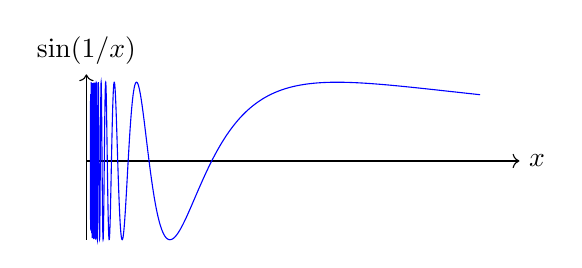
\begin{tikzpicture}[x=5cm]
            \draw[->] (0,0) -- (1.1,0) node[right] {$x$};
            \draw[->] (0,-1) -- (0,1.1) node[above] {$\sin (1/x)$};
            \draw[blue,domain=0.01:1,samples=5000] plot (\x, {sin((1/\x)r)});
        \end{tikzpicture}
        \captionof{figure}{Unit Circle in $ d_1 $}%
        \label{fig:d1-unit-circle}
    \end{minipage}
\end{example}
\begin{definition}{Advantage of path-connectedness over connectedness}{path-connect-advantage}
    The advantage of path-connectedness over connectedness is the notion of concatenation.

    Suppose a continuous function $\alpha$ connects $x$ and $y$, and a continuous function $\beta$ connects $y$ and $z$. Then, the concatenation of $\alpha$ and $\beta$ is defined by $h = \beta \times \alpha$ where
    \begin{equation}
        h(t) = 
        \begin{cases}
            \alpha(2t) & t \in [0, 1/2]\\
            \beta(2t-1) & t \in [1/2,1]
        \end{cases}
    \end{equation}
\end{definition}
\begin{theorem}{Continuous image of a path-connected set is path-connected}{cont-image-path-connect}
    If a metric space $(X,d)$ is path-connected and $f: X \to Y$ is continuous, then $f(X)\subseteq Y$ is also path-connected.

    \begin{proof}
        Omitted.
    \end{proof}
\end{theorem}
\end{document}

